\chapter{Spatial systems}\label{Spatial systems}
So far we have considered biological phenomena with negligible spatial variation. Many times, however, space is very importnant. For example, in ecological contexts you do not normally find predator and prey living together; animals often have to leave their home roosts to find food, wolves, for example.

An alternative example can be seen in the interactions of grey and red squirrels in the UK. Here, one species invades another's territory. Modelling helps us understand how the populations will evolve, \eg will one populations win out, or will the populations eventually separate the land and coexist? Equally, the modelling can inform us of how to reduce the invasive risk of the population.

There are two main forms of motion we are going to consider, random motion and directed motion.
\begin{defin}
Diffusion is the random movement of system agents. \see{Diffusion}
\end{defin}
\begin{defin}
Taxis is the directed movement of system agents. \see{Taxis}
\end{defin}
Note there are many forms of taxis, specifying what is causing the directional motion for example:
\begin{bolditemize}
\item[chemotaxis] is when the agents move up (chemoattractant) or down (chemorepellent) a chemical gradient.
\item[galvanotaxis] is movement induced by electric fields.
\item[gravitaxis] is movement that responds to gravity.
\end{bolditemize}
\begin{figure}[!!!h!!!tb]
\centering
\subfigure[\label{Diffusion}]{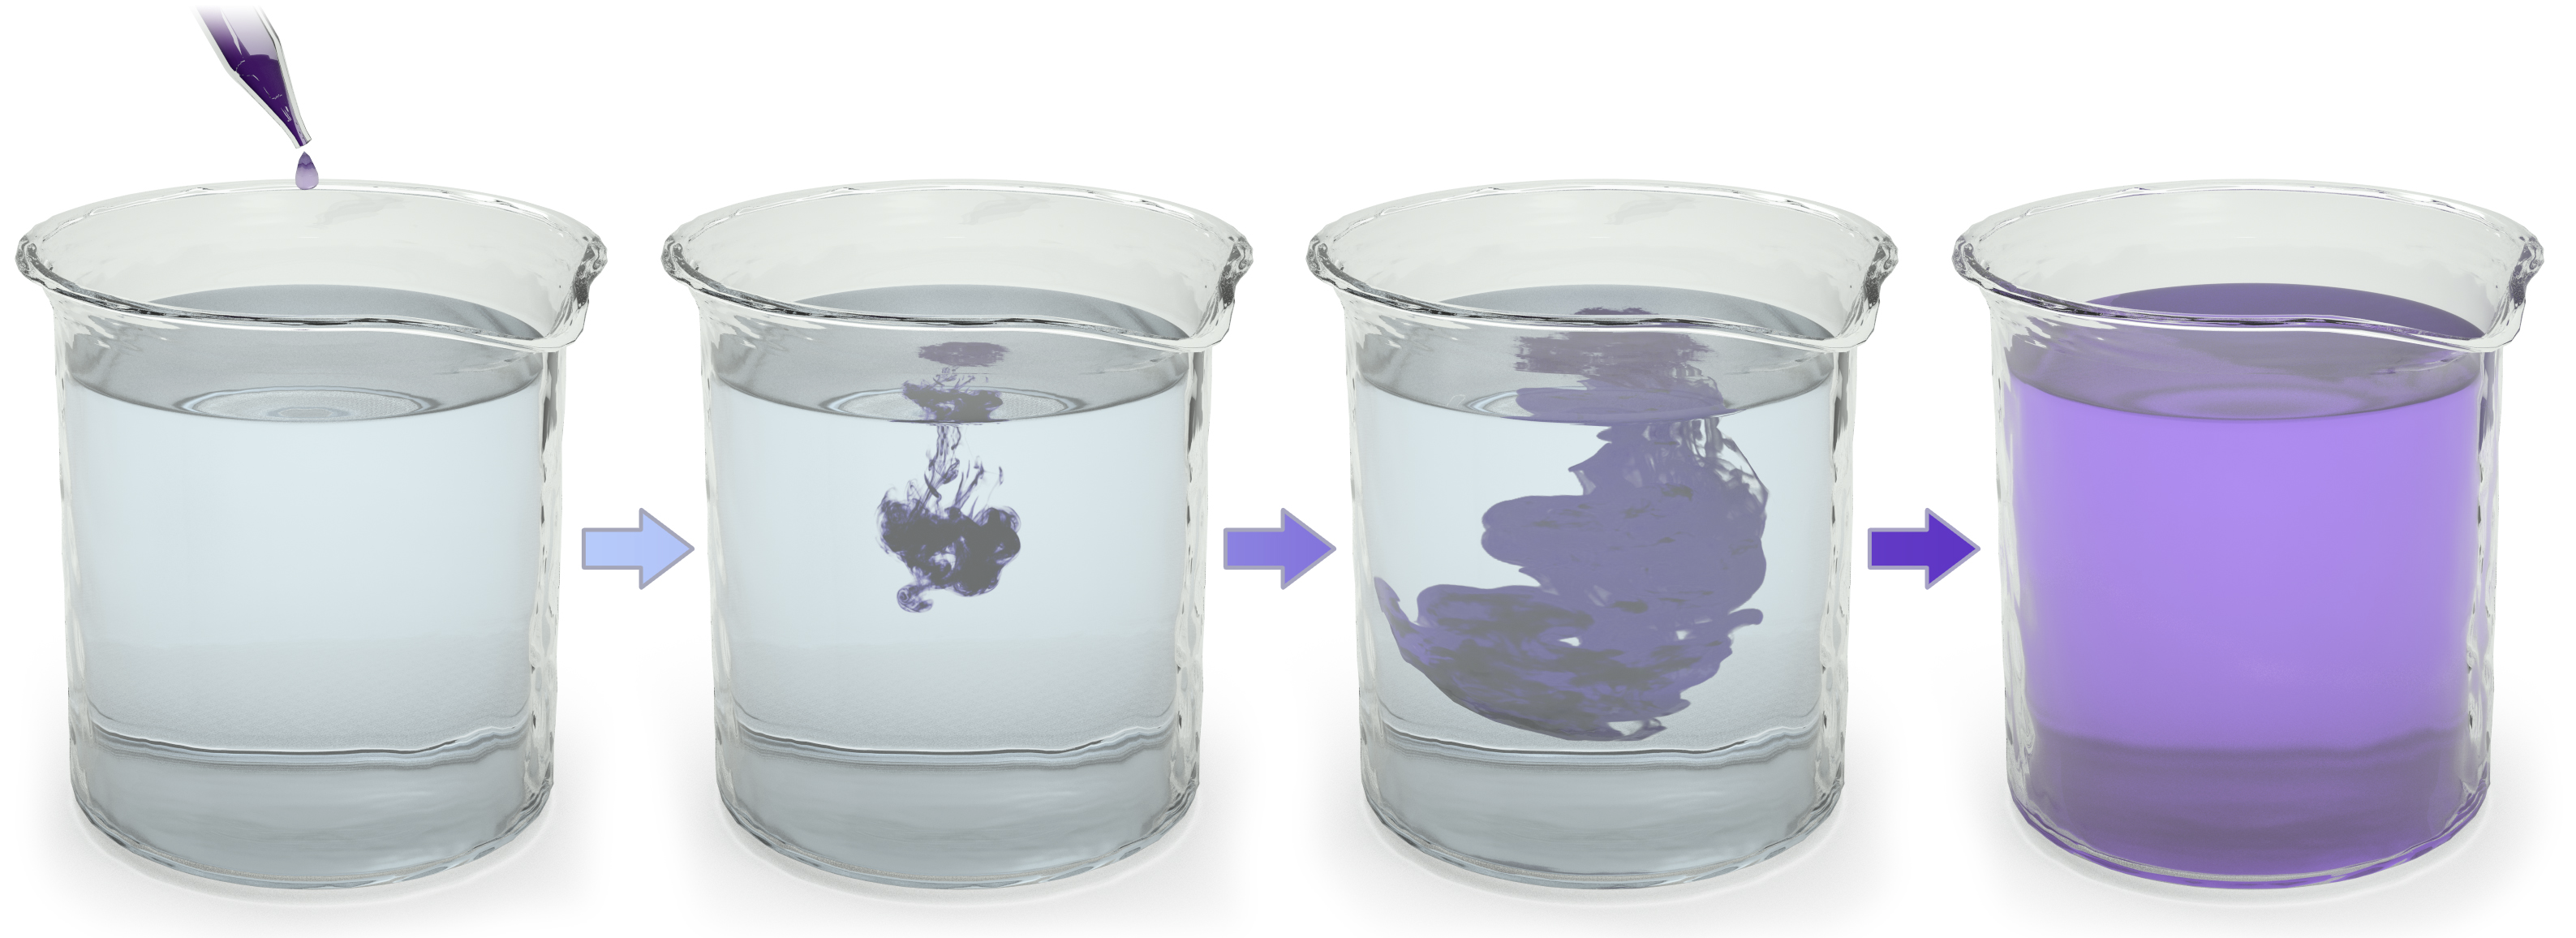
\includegraphics[width=\tp]{../Pictures/Diffusion.png}}
\subfigure[\label{Chemical_taxi}]{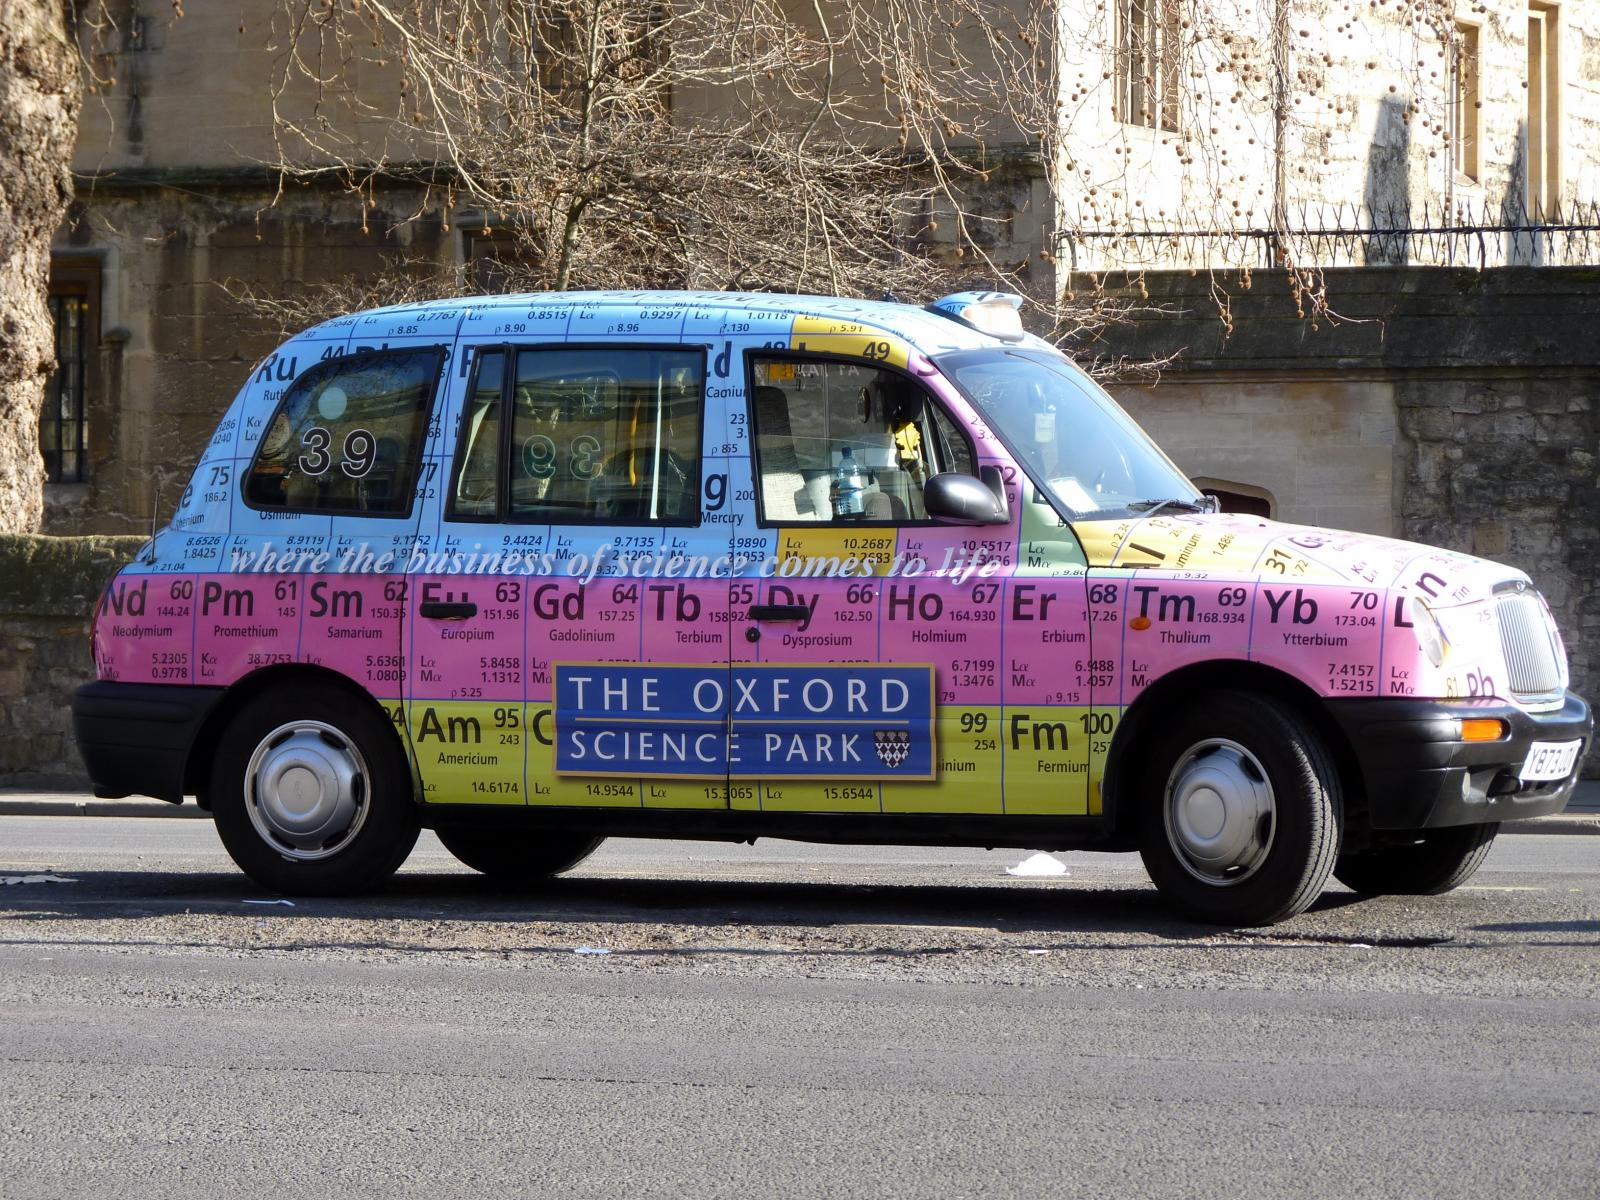
\includegraphics[height=\tttp]{../Pictures/Chemotaxis.jpg}}
\subfigure[\label{Taxis}]{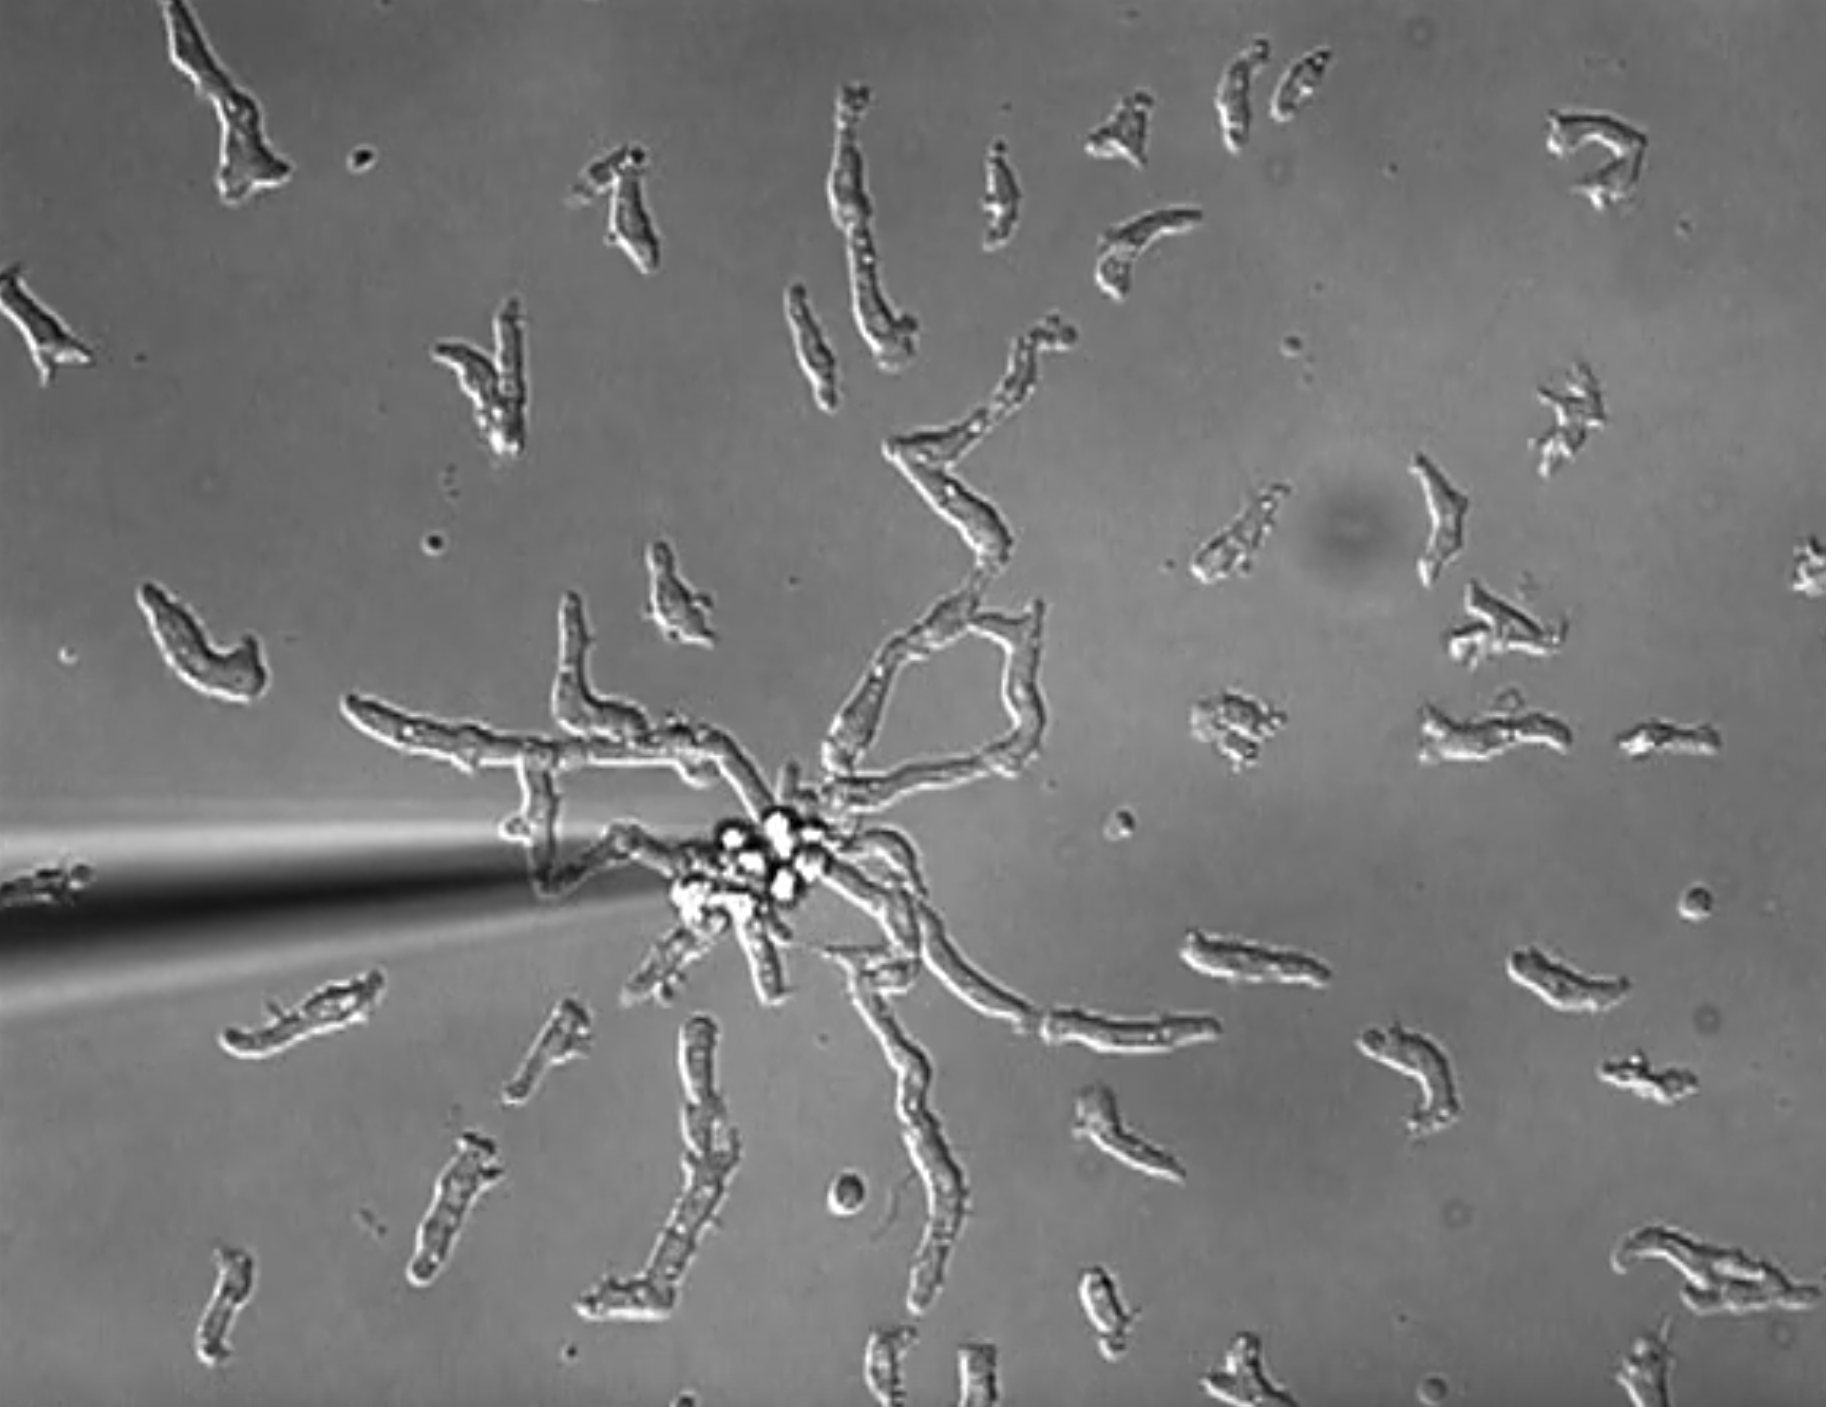
\includegraphics[height=\tttp]{../Pictures/Chemotaxis_to_cAMP.png}}
\caption{Illustrating (a) diffusion, (b) chemotaxis and (c) actual chemotaxis. In (a), as long as the water is not stirred, or heated, the ink will undergo diffusion. The ink has no directed motion, the water and ink particles bump together causing the ink to spread out to a homogeneous state. In (c) slime mould cell (dictyostelium) is attracted to a pipette full of cyclic adenosine monophosphate (cAMP). \label{Motion_types}}
\end{figure}


\section{Deriving the diffusion equation}
We will first derive the equation behind diffusion, then taxis. Further, in each case, we consider motion in the infinite domain case and then add boundaries, as these are minor complications that modify the main derivation.

All derivations follow the process of discretising a continuum population. The separation between the discretised points is then taken to zero in an appropriate limit leading to the desired equation.
\begin{thm} \label{Diffusion_derivation}
The model for random motion of a population $u$ on an infinite line  is
\bb
\D{u}{t}=D\DD{u}{x},
\ee
where $D$ is defined to be the diffusion coefficient, a positive constant that specifies the rate at which the population spreads out.

Note that since there are no boundaries we do not need to consider boundary conditions. However, an initial condition needs to be supplemented to close the model, fully. See \fig{Unbounded_diffusion} for an illustrated example.
\end{thm}
\begin{proof}
\COL{Consider an infinite one-dimensional interval on which a population, $u(x,t)$, is diffusing. Consider a discretised form of $u$ that is evaluated at points $x_i$, where $i$ is an integer label and $x_{i+1}=x_i+\Delta x$. For simplicity, $u(x_i,t)=u_i$. The population at each point is able to transition to their neighbours at a rate proportional to their concentration, with proportionality constant $d=D/\Delta x^2$. In terms of reaction terminology this is
\bb
\dots\xrightleftharpoons[d]{d}u_{i-1}\xrightleftharpoons[d]{d}u_i\xrightleftharpoons[d]{d}u_{i+1}\xrightleftharpoons[d]{d}\dots.
\ee
Due to the symmetry of the problem we can isolate just the $i^{th}$ population. Namely, using the Law of Mass Action, the accompanying infinite set of coupled ODEs would be
\bb
\D{u_i}{t}=du_{i-1}-2du_i+du_{i+1},\label{Discrete_diffusion}
\ee
where we note that we are using a partial derivative as $u$ is a function of multiple variables.

We now use Taylor's theorem to expand in $\Delta x$,
\begin{align}
&u_{i-1}=u(x_{i-1},t)=u(x_i-\Delta x,t)\approx u(x_i)-\Delta x\frac{\partial u}{\partial x}(x_i,t)+\frac{\Delta x^2}{2}\frac{\partial^2 u}{\partial x^2}(x_i,t)+h.o.t.,\label{u-}\\
&u_{i+1}=u(x_{i+1},t)=u(x_i+\Delta x,t)\approx u(x_i)+\Delta x\frac{\partial u}{\partial x}(x_i,t)+\frac{\Delta x^2}{2}\frac{\partial^2 u}{\partial x^2}(x_i,t)+h.o.t.,\label{u+}
\end{align}
where we expand to second order, rather than the normal first order.
Substituting \eqns{u+}{u-} into \eqn{Discrete_diffusion} we generate
\bb
\D{u_i}{t}=d\Delta x^2\DD{u_i}{x}.
\ee
Finally, we substitute $d=D/\Delta x^2$ and let $\Delta\rightarrow0$, at which point we stop dealing with a discretised line and consider the continuum. Thus, the diffusion equation is
\bb
\D{u}{t}=D\DD{u}{x}.
\ee}
\end{proof}
\begin{figure}[!!!h!!!tb]
\centering
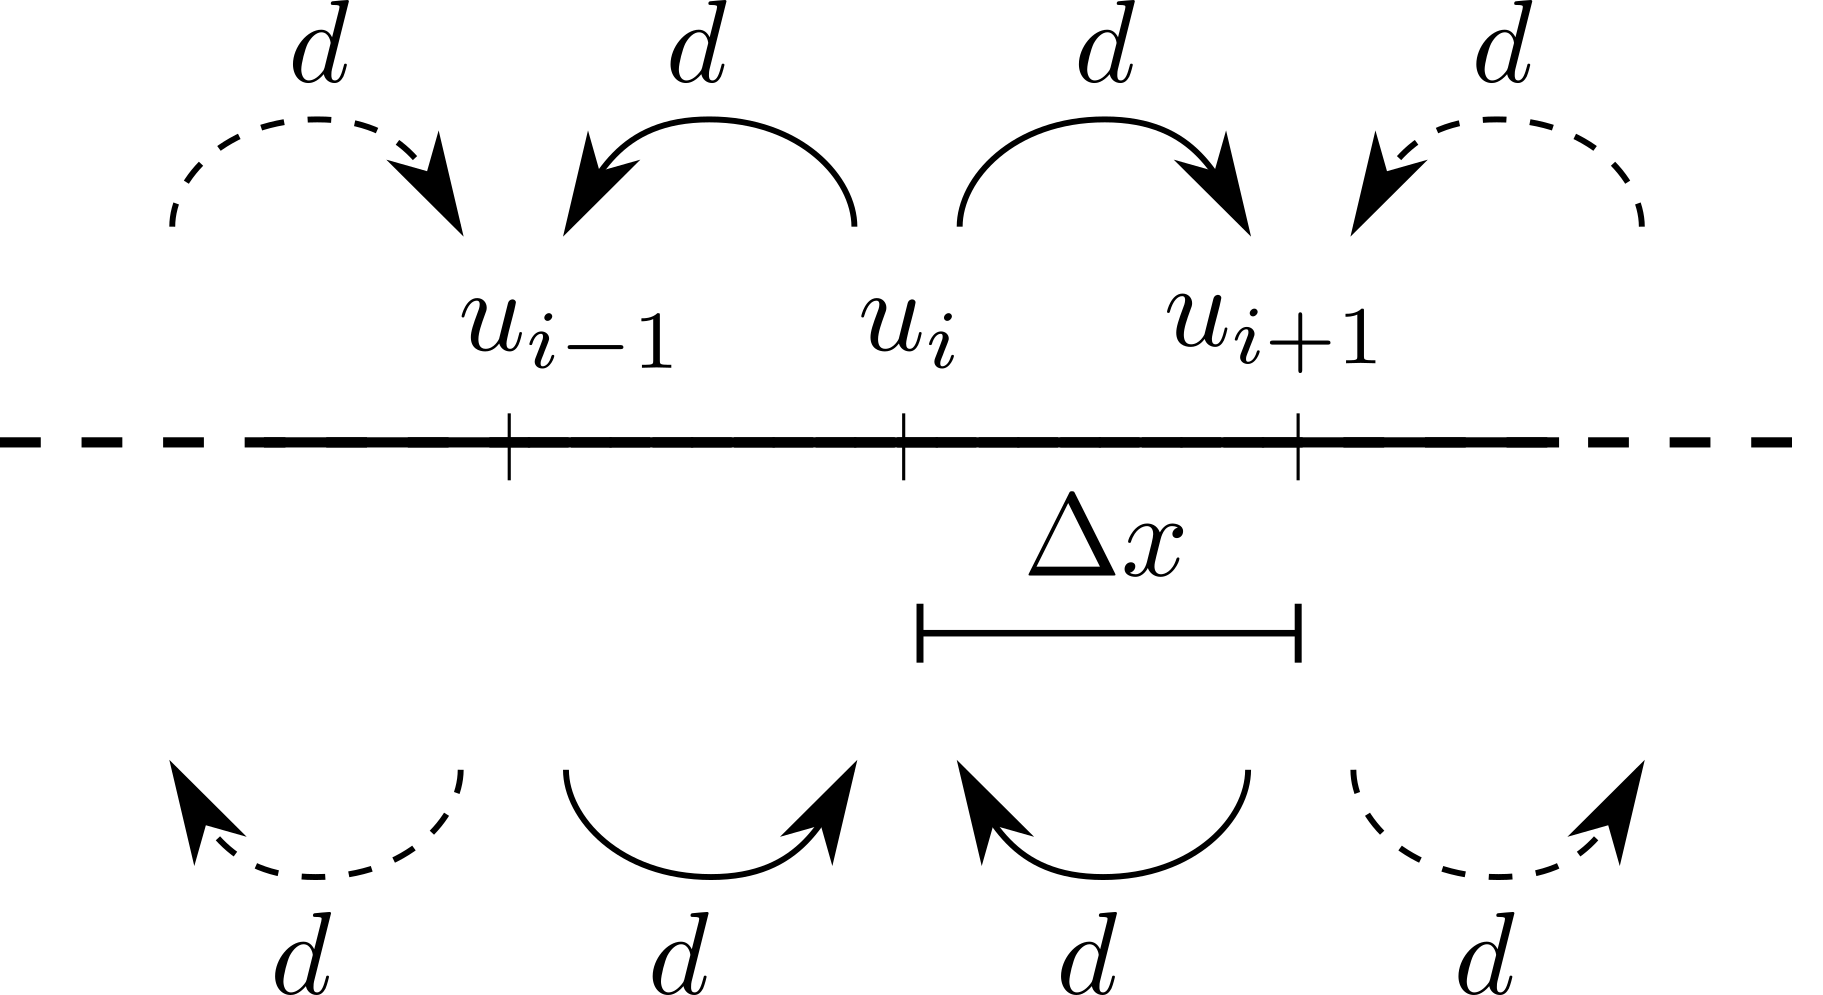
\includegraphics[width=\tp]{../Pictures/Schematic_diffusion.png}
\caption{Diffusion schematic. \label{Diffusion_schematic}}
\end{figure}
We now consider boundary conditions. Specifically, there are three main types: Dirichlet, Neumann and Robin (all named after dead mathematicians).
\begin{defin}
Dirichlet boundary conditions fix the value of the variable on the boundary to be a constant.
\end{defin}
For example, $u(0,t)=\alpha$ and $u(L,t)=\beta$, for $\alpha,\beta\geq0$ are perfectly valid Dirichlet boundary conditions for the one-dimensional diffusion equation. See \fig{Bounded_diffusion_zero_Dirichlet} for an illustrated example.
\begin{defin}
Neumann boundary conditions fix the value of the variable's derivative on the boundary to be a constant.
\end{defin}
For example,
\bb
\D{u(0,t)}{x}=\alpha \quad\text{and} \quad \D{u(L,t)}{x}=\beta\label{Neumann}
\ee
are perfectly valid Neumann boundary conditions for the one-dimensional diffusion equation.
\begin{defin}
Robin boundary conditions fix a linear combination of the  variable's value and derivative on the boundary to be a constant.
\end{defin}
For example,
\bb
\alpha_1 u(0,t)+\alpha_2\D{u(0,t)}{x}=\alpha_3 \quad\text{and} \quad \beta_1 u(L,t)+\beta_2\D{u(L,t)}{x}=\beta_3
\ee
are perfectly valid Robin boundary conditions for the one-dimensional diffusion equation.

Although there are infinitely more we will generally only consider the first two. Equally, a system is able to have different boundary conditions on each boundary.

Critically, the Neumann boundary conditions model the flux in, and out, of the domain. We will now show that when we consider an insulated domain (in which no substance enters of leave through the boundary) then we are considering the specific case of Neumann boundary conditions in which $\alpha=\beta=0$ in \eqn{Neumann}. These are specifically called zero-flux, or reflective boundary conditions.
\begin{thm}
Consider a diffusing population in a finite one-dimensional domain, $[0,L]$. Further, suppose this substance is unable to leave the domain when zero-flux boundary conditions are applied. We will show that the mathematical model of this situation is
\bb
\D{u}{t}=D\DD{u}{x},
\ee
supplemented with the boundary conditions
\bb
\D{ u(0,t)}{x}=\D{ u(L,t)}{x}=0.\label{zero-flux}
\ee
As above, an initial condition needs to be supplemented to close the model, fully. See \fig{Bounded_diffusion_zero_flux} for an illustrated example.
\end{thm}
\begin{proof}
\COL{We consider a similar set up to Theorem \ref{Diffusion_derivation}. Namely, we consider a discretised domain of $N+1$ points $\Delta x=L/N$ apart such that population $u$ evaluated at point $x_i$ is $u_i=u(x_i,t)=u(i\Delta x,t)$. However, the domain is now finite, so we explicitly specify what happens at the first and last points, $x_0=0$ and $x_N=L$ \see{Diffusion_schematic_bounded}. The reaction terms will be
\bb
u_{0}\xrightleftharpoons[d]{d}u_2\xrightleftharpoons[d]{d}\dots\xrightleftharpoons[d]{d}u_{i-1}\xrightleftharpoons[d]{d}u_i\xrightleftharpoons[d]{d}u_{i+1}\xrightleftharpoons[d]{d}\dots\xrightleftharpoons[d]{d} u_{N-1}\xrightleftharpoons[d]{d}u_{N},
\ee
which (using the Law of Mass Action) will provide an ODE system of the form
\begin{align}
\D{u_0}{t}=&du_{1}-du_0,\nonumber\\
\D{u_i}{t}=&du_{i-1}-2du_i+du_{i+1},\nonumber\\
\D{u_N}{t}=&du_{N-1}-du_N\nonumber.
\end{align}
As before we use Taylor's series (see \eqns{u-}{u+}) to generate
\begin{align}
\D{u}{t}(0)=&\frac{D}{\Delta x}\D{u}{x}(\Delta x),\label{u0}\\
\D{u_i}{t}=&D\DD{u_i}{x},\nonumber\\
\D{u}{t}(N\Delta x)=&\frac{D}{\Delta x}\D{u}{x}((N-1)\Delta x),\label{uL}
\end{align}
where we note we only have to go to first order to derive \eqns{u0}{uL}. Finally, rearranging \eqns{u0}{uL} and taking $\Delta x\rightarrow 0$ and $N\rightarrow \infty$ such that $N\Delta x=L$ stays constant, allows us to derive
\begin{align}
0=&\D{u}{x}(0),\nonumber\\
\D{u}{t}=&D\DD{u}{x},\nonumber\\
0=&\D{u}{x}(L),\nonumber
\end{align}
as required.}
\end{proof}
\begin{figure}[!!!h!!!tb]
\centering
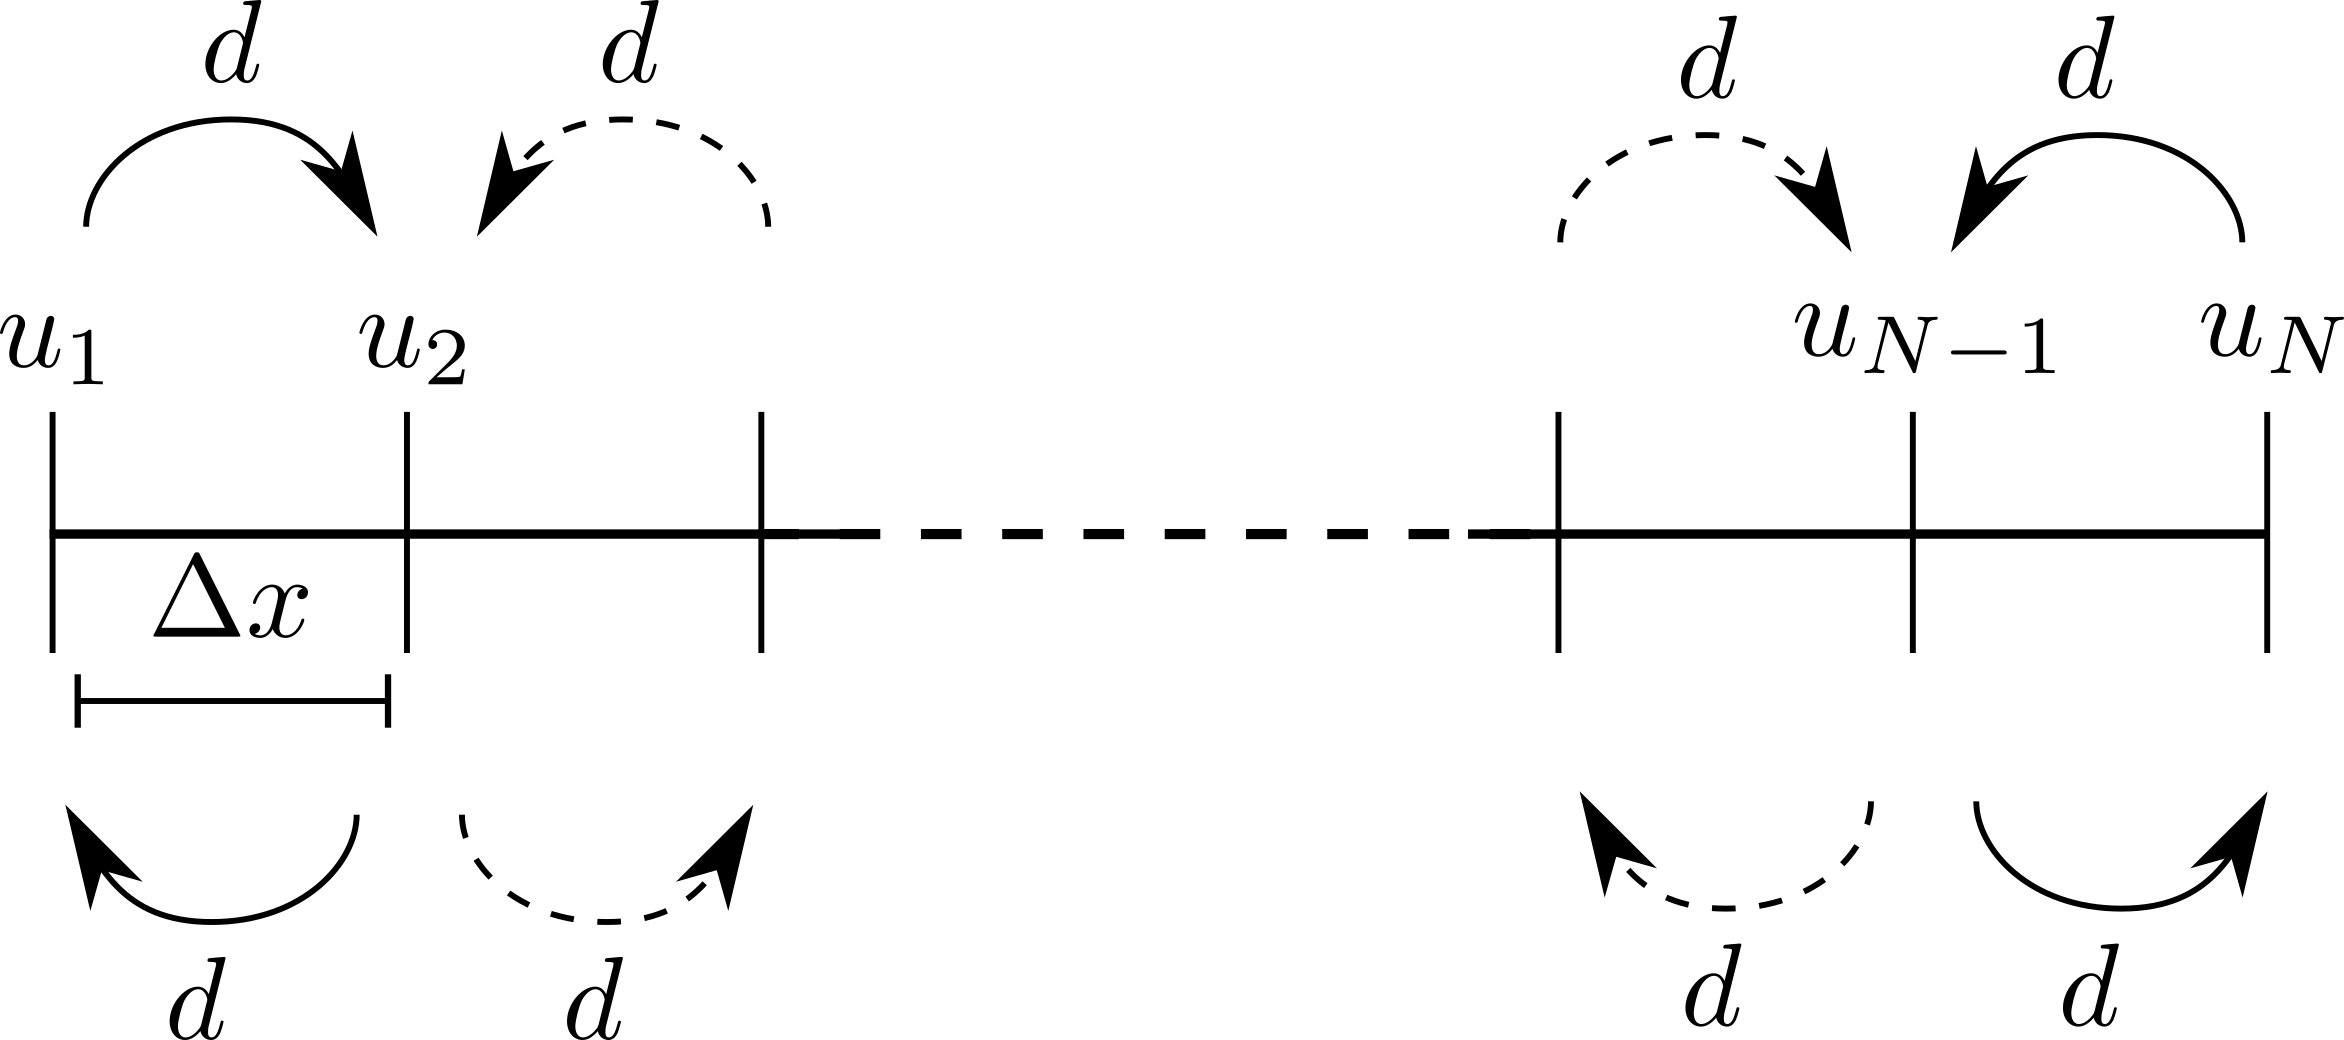
\includegraphics[width=\tp]{../Pictures/Schematic_diffusion_bounded.png}
\caption{Diffusion schematic within an insulated domain. \label{Diffusion_schematic_bounded}}
\end{figure}
\begin{thm}
Consider a one-dimensional diffusing population. In the case of a zero-flux boundary conditions, the population total does not change.
\end{thm}
\begin{proof}
\COL{Intuitively, this makes sense as the population is simply spreading out over the domain. No population is being created or destroyed. Nor is any allowed to leave the domain in the finite interval case. Thus, we would hope that this were true.

To show that the proposition is true we simply integrate the population over space and demonstrate that its time derivative is zero. Hence, the population remains constant over time. Namely, we begin by integrating the diffusion equation between $L_0$ and $L\infty$,
\bb
\int^{L_\infty}_{L_0}\D{u}{t}\rd x=\int^{L_\infty}_{L_0}D\DD{u}{x}\rd x.\label{Integrated_diffusion}\\
\ee
The time derivative and spatial integration commute and we can directly integrate the right-hand side of \eqn{Integrated_diffusion}. We, thus, derive
\bb
\frac{\rd }{\rd t}\int^{L_\infty}_{L_0}u\rd x=D\left[\D{u}{x}\right]^{L_\infty}_{L_0}\label{Total_u},
\ee
where the left-hand side of \eqn{Total_u} is the time derivative of the total amount of $u$ in the domain 
%and the right-hand side is zero in both cases of an infinite domain, or zero-flux boundary conditions.
%
%Specifically, in the infinite domain case we require a bounded solution, thus,
%\bb
%\D{u}{x}(L_0) \rightarrow 0 \text{ as } L_0\rightarrow-\infty\text{ and }\D{u}{x}(L_\infty) \rightarrow 0\text{ as }L_\infty\rightarrow \infty
%\ee
and the derivatives are explicitly zero in the zero-flux case (see \eqn{zero-flux}).}
\end{proof}
\begin{figure}[!!!h!!!tb]
\centering
\subfigure[\label{Unbounded_diffusion}]{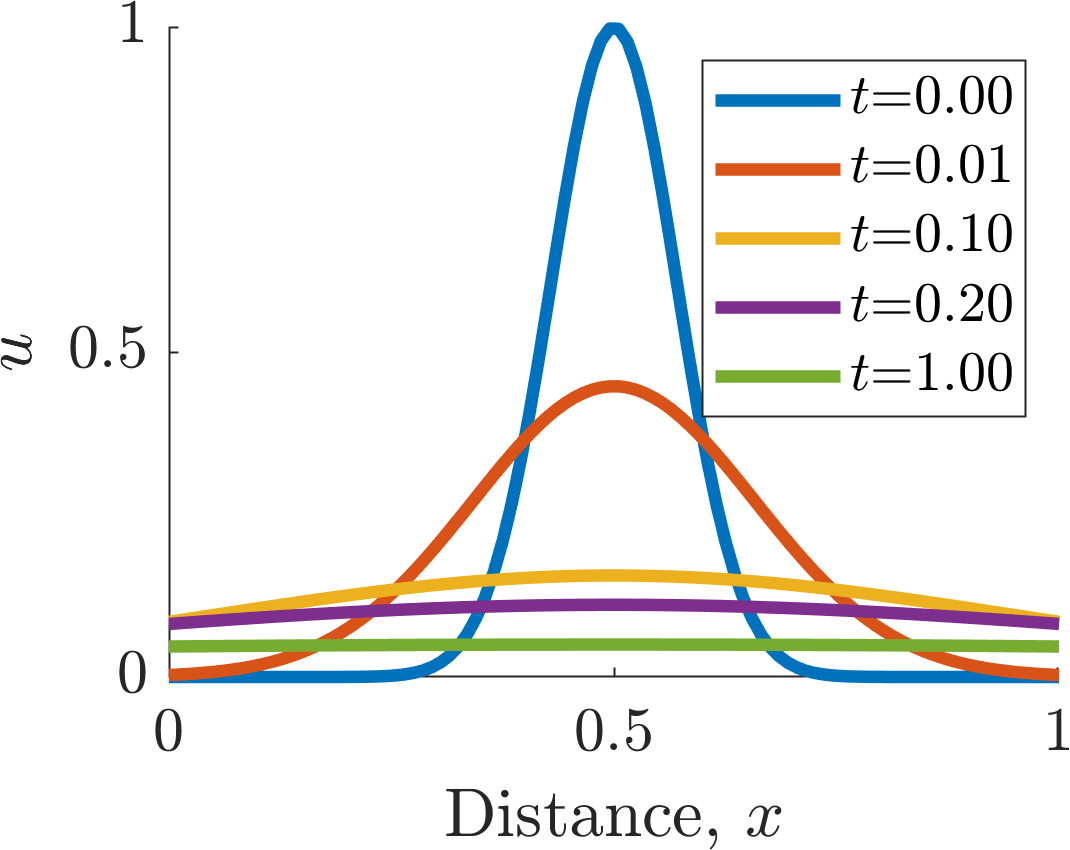
\includegraphics[width=\tttp]{../Pictures/Unbounded_diffusion.png}}
\subfigure[\label{Bounded_diffusion_zero_flux}]{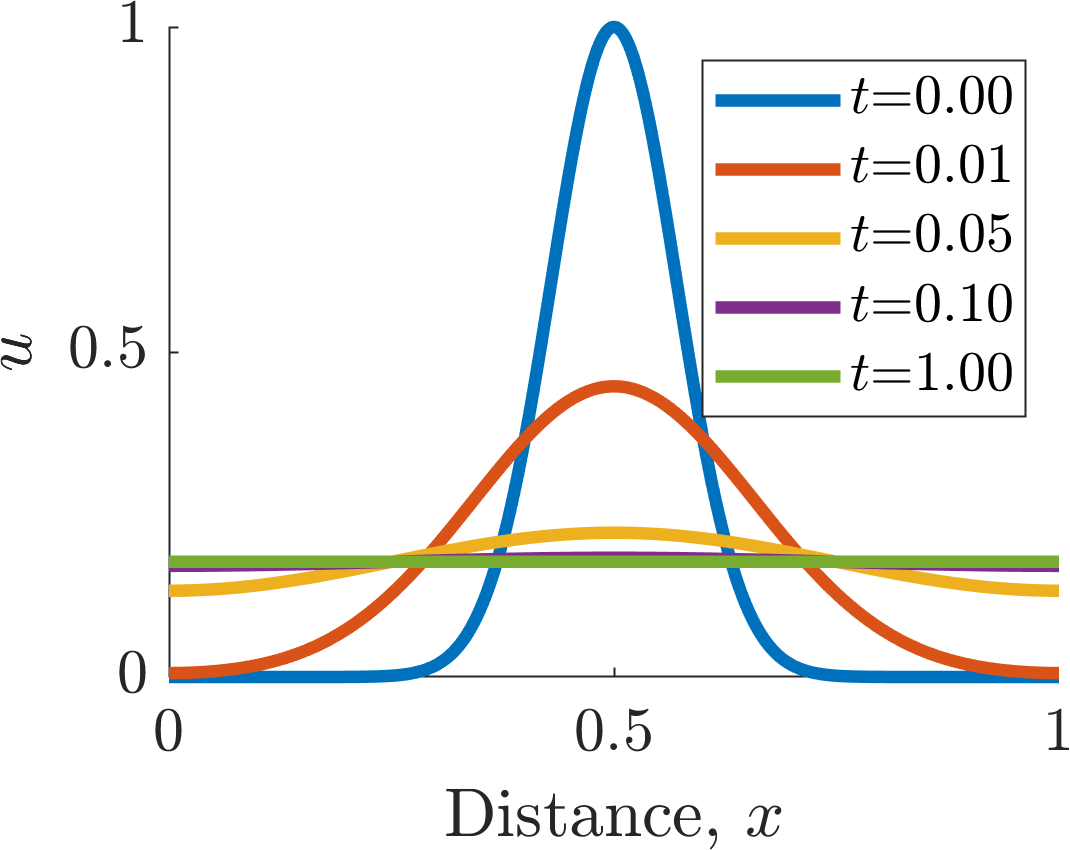
\includegraphics[width=\tttp]{../Pictures/Bounded_diffusion_zero_flux}}
\subfigure[\label{Bounded_diffusion_zero_Dirichlet}]{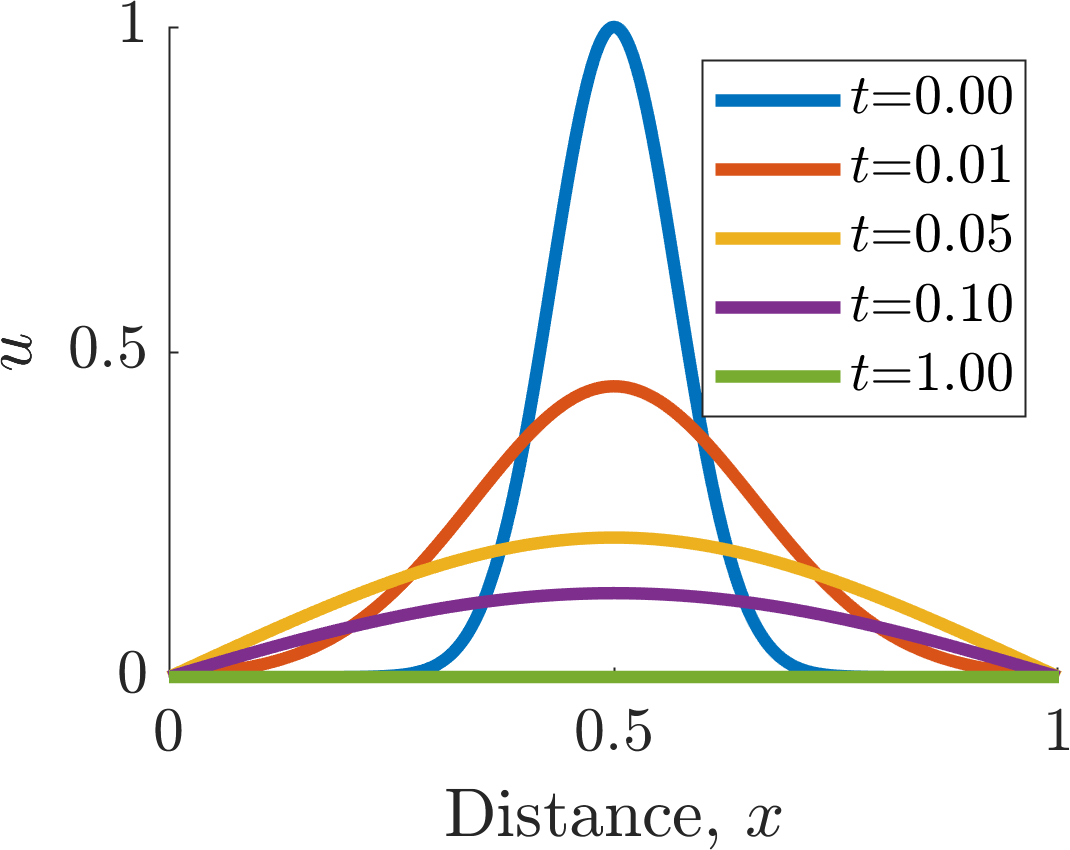
\includegraphics[width=\tttp]{../Pictures/Bounded_diffusion_zero_Dirichlet}}
\caption{Illustrating diffusion on (a) an infinite domain, (b) a finite domain with zero-flux boundaries and (c) a finite domain with zero-Dirichlet boundaries. Parameter value $D=1$ in all cases. The initial condition in all cases was $u(x,0) = \exp(-((x-1/2)10)^2)$.\label{Diffusion_images}}
\end{figure}
\section{Deriving the taxis equation}
In the last section we saw that the diffusion equation required the second spatial derivative. The derivation of the taxis equations follow exactly the same argument, but we will see that the taxis equation only requires the first spatial derivative. This is simpler to derive, but we started with the more complicated equation because we will be using diffusion more often and it was important to get ourselves used to the derivation argument.
\begin{thm}
Consider a one-dimensional domain filled with a population $u$ that is subject to two different spatially dependent forces. One force attracts the population to the left, causing a flux of movement at a rate, $d_l(x)=D_l(x)/\Delta x$, whilst the other attracts the population to the right, causing a flux of movement at a rate $d_r(x)=D_r(x)/\Delta x$. The equation controlling the populations evolution is then
\bb
\D{u}{t}=\D{\l[ D_l(x)-D_r(x)] u\r}{x}.
\ee
Since we are on an infinite domain we simply have to assume that the solution stays finite and initial conditions are required to close the solution.
\end{thm}
\begin{proof}
\COL{Consider the standard set up. Namely, consider a discretised population $u$ where each point is separated by $\Delta x$ containing a population \see{Taxis_schematic}. The reaction terms will be
\bb
\dots\xrightleftharpoons[d_l(x_{i-1})]{d_r(x_{i-2})}u_{i-1}\xrightleftharpoons[d_l(x_i)]{d_r(x_{i-1})}u_i\xrightleftharpoons[d_l(x_{i+1})]{d_r(x_{i})}u_{i+1}\xrightleftharpoons[d_l(x_{i+2})]{d_r(x_{i+1})}\dots,
\ee
which (using the Law of Mass Action) will provide an ODE system of the form
\begin{align}
\D{u_i}{t}=&d_l(x_{i+1})u_{i+1}-d_l(x_i)u_i+d_r(x_{i-1})u_{i-1}-d_r(x_{i})u_{i},\label{Taxis_eqn}
\end{align}
As before we use Taylor's series. Although we only need to expand to first order, we need to expand both the movement rates and the positions,
\begin{align}
&d_l(x_{i+1})=d_l(x_{i}+\Delta x)\approx d_l(x_i)+\Delta x\D{d_l}{x}+h.o.t,\label{dl}\\
&d_r(x_{i-1})=d_r(x_{i}-\Delta x)\approx d_r(x_i)-\Delta x\D{d_r}{x}+h.o.t,\\
&u_{i-1}=u(x_i-\Delta x,t)\approx u(x_i)-\Delta x\frac{\partial u}{\partial x}+h.o.t.,\\
&u_{i+1}=u(x_i+\Delta x,t)\approx u(x_i)+\Delta x\frac{\partial u}{\partial x}+h.o.t..\label{u+1}
\end{align}
Substituting \eqnto{dl}{u+1} into \eqn{Taxis_eqn} gives
\begin{align}
\D{u_i}{t}\approx&\l d_l(x_i)+\Delta x\D{d_l}{x}\r\l u(x_i)+\Delta x\frac{\partial u}{\partial x}\r-d_l(x_i)u_i\nonumber\\
&+\l d_r(x_i)-\Delta x\D{d_r}{x} \r\l u(x_i)-\Delta x\frac{\partial u}{\partial x}\r-d_r(x_{i})u_{i}\nonumber\\
\approx&\Delta x u_i\D{d_l}{x}+\Delta x d_l(x_i)\D{u_i}{x}-\Delta x u_i\D{d_r}{x}-\Delta x d_l(x_i)\D{u_i}{x},\nonumber\\
\approx&u_i\l\D{D_l}{x}-\D{D_r}{x}\r+\l D_l(x_i)- D_r(x_i)\r\D{u_i}{x},\nonumber\\
\approx&\D{\l [D_l(x_i)- D_r(x_i)] u_i\r}{x}.\nonumber
\end{align}
Upon taking $\Delta x\rightarrow 0$ we achieve the stated result.}
\end{proof}
\begin{figure}[!!!h!!!tb]
\centering
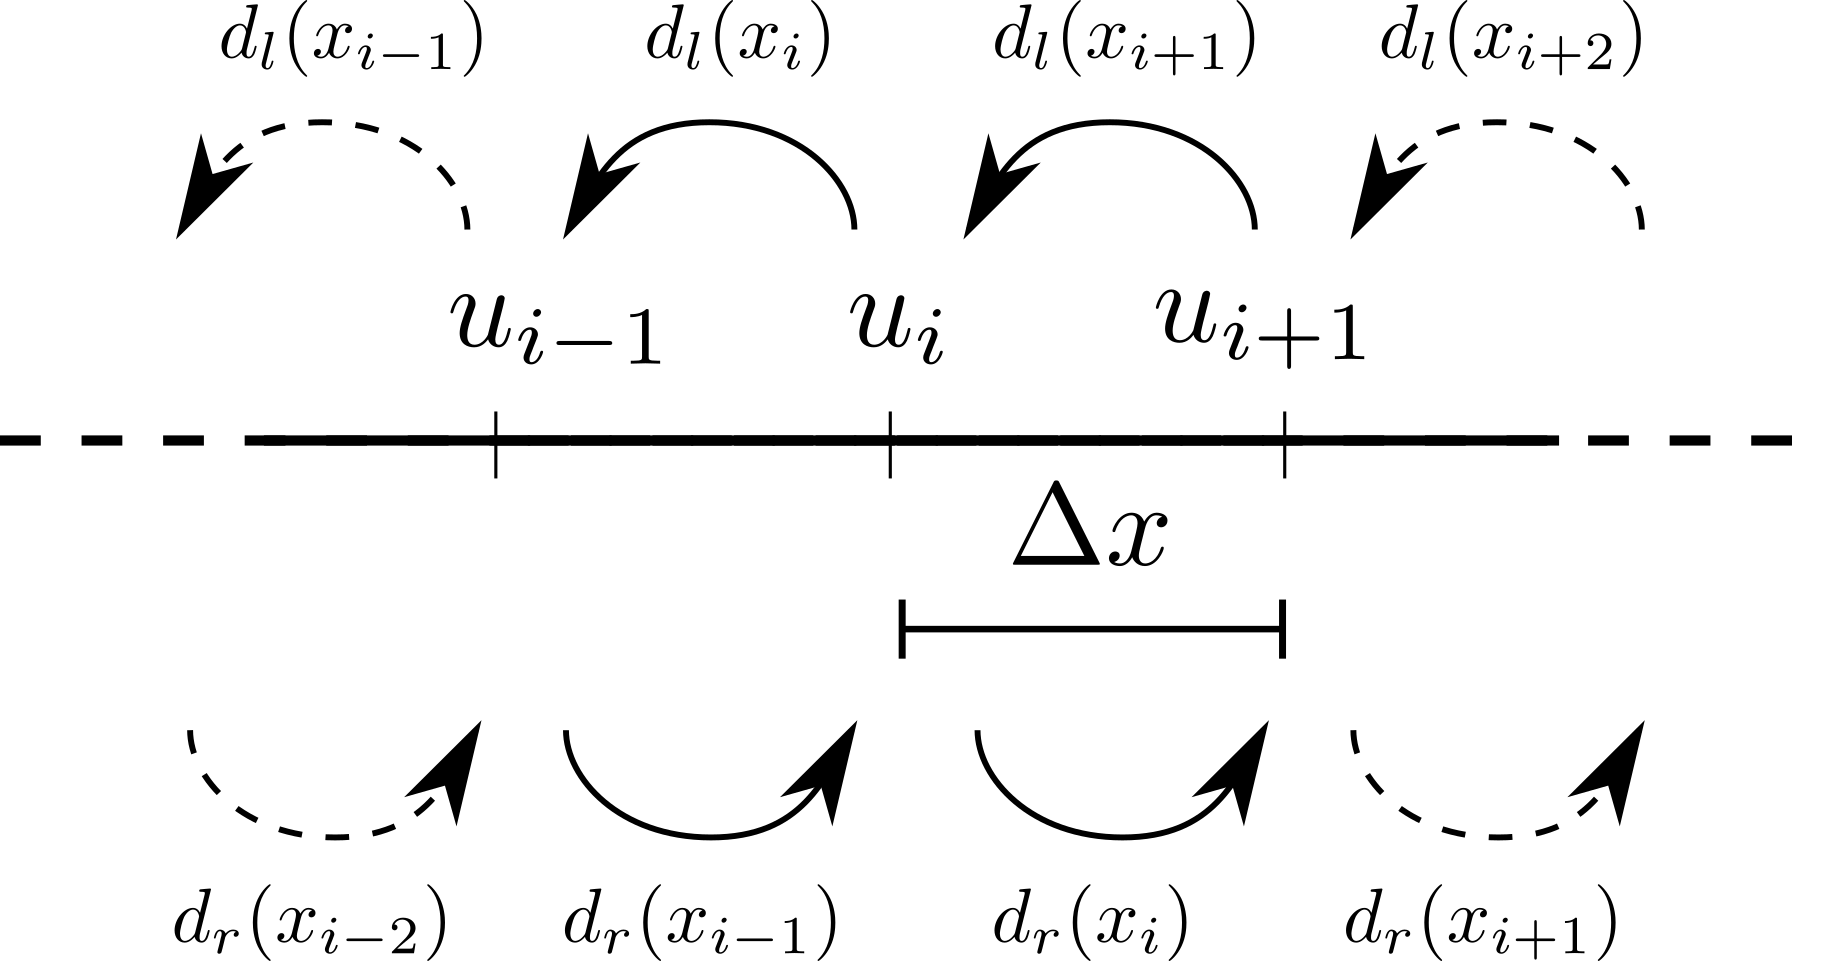
\includegraphics[width=\tp]{../Pictures/Schematic_taxis.png}
\caption{Taxis schematic. \label{Taxis_schematic}}
\end{figure}
\begin{figure}[!!!h!!!tb]
\centering
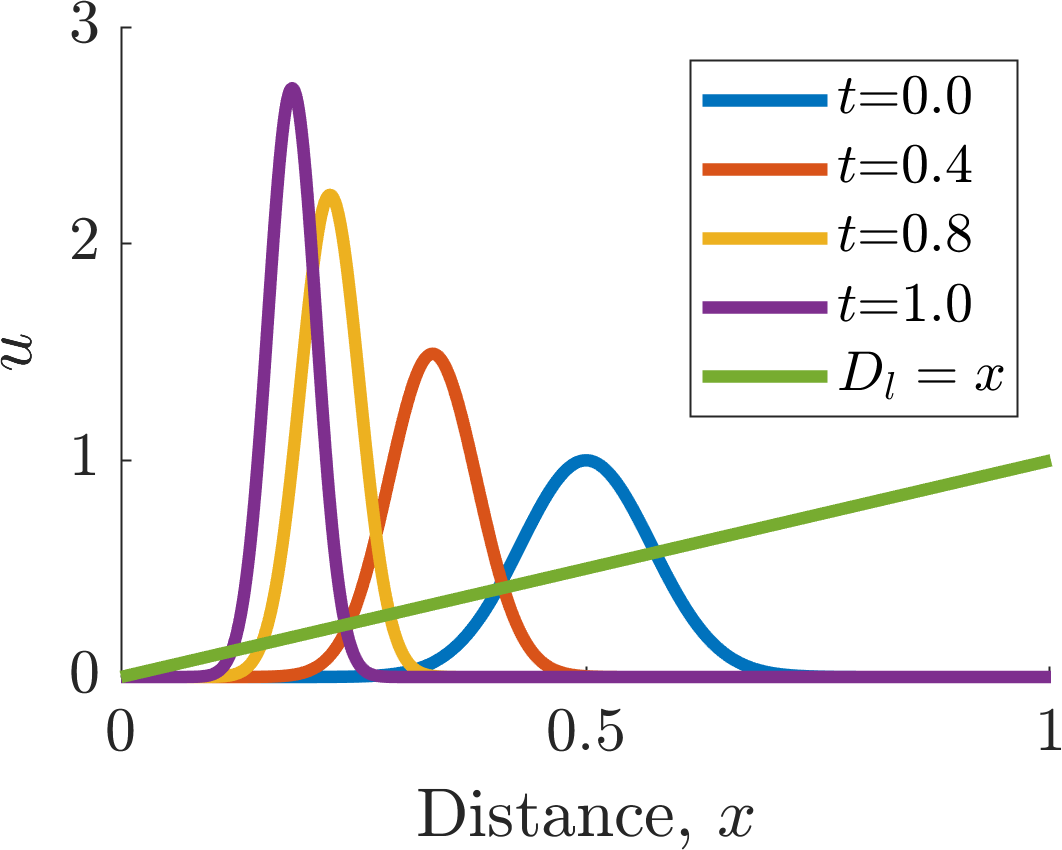
\includegraphics[width=\ttp]{../Pictures/Taxis.png}
\caption{Illustrating taxis on a finite domain with zero-flux boundary conditions with $D_l=x$ and initial condition $u(x,0)=\exp(-((x-0.5)10)^2)$. }
\end{figure}
\section{Travelling waves}
In previous chapters we have developed a theoretical framework of interacting species. Such interactions can simply be added to models of spatial motion. Namely, if $f(u,v)$ and $g(u,v)$ are interaction kinetics for populations $u$ and $v$ then
\begin{align}
\D{u}{t}=&D_u\DD{u}{x}+f(u,v),\\
\D{v}{t}=&D_v\DD{v}{x}+g(u,v),
\end{align}
would be a one-dimensional spatial extension of the reaction kinetics, assuming that populations $u$ and $v$ diffused with rates $D_u$ and $D_v$, respectively.

However, before we consider the possibilities of two interacting populations, we consider the simple example of combining logistic growth and diffusion in one spatial dimension. Critically we are going to look conditions under which \textit{Fisher waves} can form
\begin{defin}\label{Fisher_wave}
A Fisher wave is a specific form of travelling wave solution that translates in space at a constant speed over time, without changing its shape.
\end{defin}

\subsection{Fisher's equation}
\begin{example}[frametitle=Fisher waves in Fisher's Equation]
Consider the following system
\bb
\D{u}{t}=D\DD{u}{x}+ru\l 1-\frac{u}{K}\r,\label{Fisher}
\ee
on an infinite domain, subject to the following boundary and initial conditions:
\bb
u(x,t)\rightarrow u_{\pm\infty} \textrm{ as } x\rightarrow \pm\infty \textrm{ and }u(x,0)=u_0(x).\label{bcs_ics}
\ee
where $u_{\pm \infty}$ are constants to be determined and $u_0(x)$ is any function satisfying the boundary conditions. This equation is known as Fisher's equation and it was first proposed to model the spread of an advantageous gene through a population.

We will show that Fisher waves, as defined in definition \eqn{Fisher_wave}, can be supported by \eqn{Fisher}. We  will be led by our intuition of what we expect the waveform to look like \see{Fisher_wave_fig}. Namely, from our understanding of the logistic equation any small perturbation to zero leads the population to grow to the carrying capacity. Thus, we expect that large populations  will invade small populations until everywhere is at $u=K$.

\begin{enumerate}
\item \COL{We, firstly, need to derive what boundary conditions would be consistent with \eqn{bcs_ics}. Since $u_{\pm\infty}$ are constant ``at infinity'' this means the spatial and temporal derivatives are zero at the boundaries. Namely, the values must satisfy
\bb
0=u_{\pm\infty}\l 1-\frac{u_{\pm\infty}}{K} \r.
\ee}
\COL{Thus, $u_{\pm\infty}=0$, or $K$, meaning that the final solution forms are heavily restricted in what their boundary values can be.}

\item \COL{We want the wave-form solution to move with constant speed. This suggests that we convert to using moving wave coordinates, $z=x-ct$, where $z$ is travelling wave coordinate and $c$ is a constant velocity. Note that we assume without loss of generality that $c>0$. If $c<0$ then the wave is simply going in the opposite direction. Critically, we have introduced a new variable and, thus, we must derive conditions on the form $c$ must take.

Using $z=x-ct$ the derivatives become
\begin{align}
\D{u}{t}=&\D{u}{z}\D{z}{t}+\D{u}{t}\D{t}{t},\nonumber\\
=&-c\D{u}{z}+\D{u}{t},\label{dtdz}
\end{align}
and
\begin{align}
\D{u}{x}=&\D{u}{z}\D{z}{x}+\D{u}{x}\D{t}{x},\nonumber\\
=&\D{u}{z},\nonumber\\
\implies \DD{u}{x}=&\DD{u}{z}.\label{dxdz}
\end{align}
Substituting \eqns{dtdz}{dxdz} in \eqn{Fisher} we generate
\bb
\D{u}{t}-c\D{u}{z}=D\DD{u}{z}+ru\l 1-\frac{u}{K} \r.
\ee
Equally, we want the wave to move without it changing its shape. This means that the wave should be stationary in the moving coordinates, \ie $\partial u/\partial t=0$. Thus, the travelling wave solution satisfies
\bb
0=D\frac{\rd^2 u}{\rd z^2}+c\frac{\rd u}{\rd z}+ru\l 1-\frac{u}{K} \r.\label{Travelling_wave}
\ee
and we choose boundary conditions
\bb
u(-\infty)=K, \quad u(\infty)=0.
\ee
Namely, far ahead of the wave there is no population, whilst behind the wave the population is at carrying capacity.}


\item \COL{Using the substitution $v=\partial u/\partial z$, we now consider \eqn{Travelling_wave} as a system of two first order ODEs
\begin{align}
\frac{\rd u}{\rd z}=&v,\label{Fisher_u}\\
D\frac{\rd v}{\rd z}=&-cv-ru\l 1-\frac{u}{K} \r.\label{Fisher_v}
\end{align}
The steady states of these are $(0,0)$ and $(K,0)$. The Jacobian of the system is
\bb
\bm{J}=\left[ \begin {array}{cc} 
0 &1\\
 r(2u_s/K-1)/D&-c/D\end {array}\\
   \right].
\ee}
\COL{The eigenvalues satisfy
\bb
-\lambda\l -\frac{c}{D}-\lambda\r-\frac{r}{D}\l 2\frac{u_s}{K}-1\r =0,
\ee
and, so,
%l^2+cl-r(2u/K-1)
\bb
\lambda_{\pm}=\frac{-c\pm\sqrt{c^2+4rD(2u_s/K-1)}}{2D},
\ee
where we note that the eigenvalues depend only on the steady state value of $u$, not $v$. Evaluating these eigenvalues at the steady states we get
\bb
\lambda_{\pm}(K,0)=\frac{-c\pm\sqrt{c^2+4Dr}}{2},\quad\lambda_{\pm}(0,0)=\frac{-c\pm\sqrt{c^2-4Dr}}{2}.
\ee
Since $c,r,D>0$ then $\lambda_{-}(K,0)<0<\lambda_{+}(K,0)$ and, hence, $(K,0)$ is a saddle point. Equally, $Re(\lambda_{\pm}(0,0))<0$, so $(0,0)$ is a stable point. However, depending on how large $r$ is it could either be a stable node, or a stable spiral.

However, if $(0,0)$ were a spiral point it would mean that $u$ would become negative, but $u$ is a physical population and, so, this cannot happen. Thus, we require $(0,0)$ to be a stable node and, hence, we need $c^2\geq 4Dr$.}

\item \COL{Finally, to show that the wave form is possible we need to show that there is a trajectory linking $(K,0)$ to $(0,0)$. Since $(K,0)$ is unstable and $(0,0)$ is stable, it is suggestive, but we still need to show that it is possible. To do this we construct a trapping region, $R$, which will contain both critical points. The trajectory will enter $R$ from $(K,0)$ and will be unable to leave. We then depend on The Poincar\'e-Bendixson Theorem to tell us what will happen.}
\begin{thm}[The Poincar\'e-Bendixson Theorem]
For a system of two first order ordinary differential equations, consider a closed bounded
region, $R$. Suppose a trajectory, $\bm{p}(t)=(u(t),v(t))$, lies entirely within $R$. Then one of the
following is true:
\begin{enumerate}
\item $\bm{p}(t)$ is a closed trajectory, \eg a limit cycle;
\item $\bm{p}(t)$ asymptotically tends to a closed trajectory, \eg a limit cycle;
\item $\bm{p}(t)$ terminates at a stationary point.
\end{enumerate}
Therefore, if $R$ does not have a stationary point then there must be a limit cycle. Equally, if $R$ does not contain a limit cycle then the trajectory must terminate.
\end{thm}
\begin{proof}
Nonexaminable, but, for the interested, see P. Glendinning, Stability, Instability and Chaos: An Introduction to the Theory of Nonlinear Differential Equations.
\end{proof}
\COL{Using The Poincar\'e-Bendixson Theorem we will show that $R$ cannot contain a limit cycle and, thus, the trajectory, must terminate at $(0,0)$. Thereby providing us with a waveform solution that links $(K,0)$ to $(0,0)$.}

\COL{We begin by considering the direction of the trajectory on the line $v=-cu/(2D)$, for} \COL{$0<u<K$,
\begin{align}
\frac{\rd v}{\rd u}=&\frac{-cv-ru\l 1-\frac{u}{K}\r }{Dv},\nonumber\\
=&-\frac{c}{D}-\frac{ru\l 1-\frac{u}{K}\r }{Dv},\nonumber\\
=&-\frac{c}{D}+\frac{2r\l 1-\frac{u}{K}\r }{c},\nonumber\\
=&-\frac{c}{D}+\frac{2r}{c}-\frac{2ru}{Kc},\nonumber\\
<&-\frac{c}{D}+\frac{2r}{c} \textrm{ whenever $0<u<K$}. \label{Dynamic_direction}
\end{align}
For a wave to exist we have shown that $c^2>4Dr$, or $c/(2D)>2r/c$. Substituting this into \eqn{Dynamic_direction} we get that
\begin{align}
\frac{\rd v}{\rd u}<&-\frac{c}{D}+\frac{2r}{c},\nonumber\\
<&-\frac{c}{D}+\frac{c}{2D},\nonumber\\
=&-\frac{c}{2D}.\label{Dynamic_direction2}
\end{align}
Using this we construct a triangular region, $R$
such that
\bb
R=\{(u,v): 0\leq u\leq K, -\frac{cu}{2D}<v<0\}
\ee
and consider the $(u,v)$ phase plane \see{Fisher_phase_plane}. Firstly, we construct the nullclines
\begin{align}
v=&0,\\
v=&\frac{r}{c}u\l \frac{u}{K}-1\r,
\end{align}
(blue lines in \fig{Fisher_phase_plane}) then we consider the sign of each derivative in the different sectors, and on the nullclines and use these to draw in the directional arrows (black and blue arrows, respectively).

Next, we draw the $R$ region and consider the direction of the dynamics on each of the boundaries. By the derivation of inequality \eqref{Dynamic_direction2} we know that the directional arrows are always steeper than the line $v=-cu/(2D)$, thus, trajectories inside $R$ cannot leave via the hypotenuse. For $v=0$, $0\leq u\leq K$ we have that  $u'=0$ and $v'<0$ so, again, the trajectory cannot leave via the horizontal section of $R$. When $u=K$ and $v\leq0$ we have that $u'<0$ and $v'>0$, which once again points into $R$ and, thus, once a trajectory enters $R$ it cannot escape via the side.

Finally, we know a limit cycle cannot exist in $R$ as $u'\leq 0$ at every point in $R$. However, if the trajectory were to cycle the values must increase, as well as decrease, which is not possible. Thus, by The Poincar\'e-Bendixson Theorem the trajectory must terminate at a steady state and $(0,0)$ is the only candidate.

Hence, we have demonstrated that a trajectory linking $(K,0)$ to $(0,0)$ is possible. A possible trajectory is shown in green in \fig{Fisher_phase_plane}.}

\item \COL{Note that we have shown a Fisher wave is possible in \eqn{Fisher}. We have not shown that it is guaranteed. However, as you might expect, Fisher waves do generically appear in the Fisher equation. Proving this is beyond this course. However, we can simulate \eqn{Fisher} and demonstrate that our assumptions and intuition do hold. Firstly, compare \fig{Fisher_wave_fig} and the left subfigure of \fig{Fisher_sims}. Here, we see that apart from near the boundaries\footnote{Although our mathematics is specifically for an infinite domain, we, of course, cannot simulate this. Thus, often mathematicians simulate ``large'' domains and consider the solution far away from the boundaries. However, what ``large'' means is heavily context dependent.} the wave does propagate with a constant wave form shape. Equally, by comparing \fig{Fisher_phase_plane} and the middle subfigure of \fig{Fisher_sims} we can see that the trajectory of the solution of \eqn{Fisher} does follow the $(u,v)$ phase plane of \eqn{Travelling_wave}. Finally, the \fig{Fisher_sims} demonstrates that the wave does travel with a constant rate (away from the boundaries). }\COL{Critically, our maths provides only the inequality $c\geq\sqrt{4Dr}=\sqrt{4\times 1\times 4}=4$. Our maths does not predict the general observation that $c\rightarrow\sqrt{Dr}$.}
\end{enumerate}
\end{example}
\begin{figure}[!!!h!!!tb]
\centering
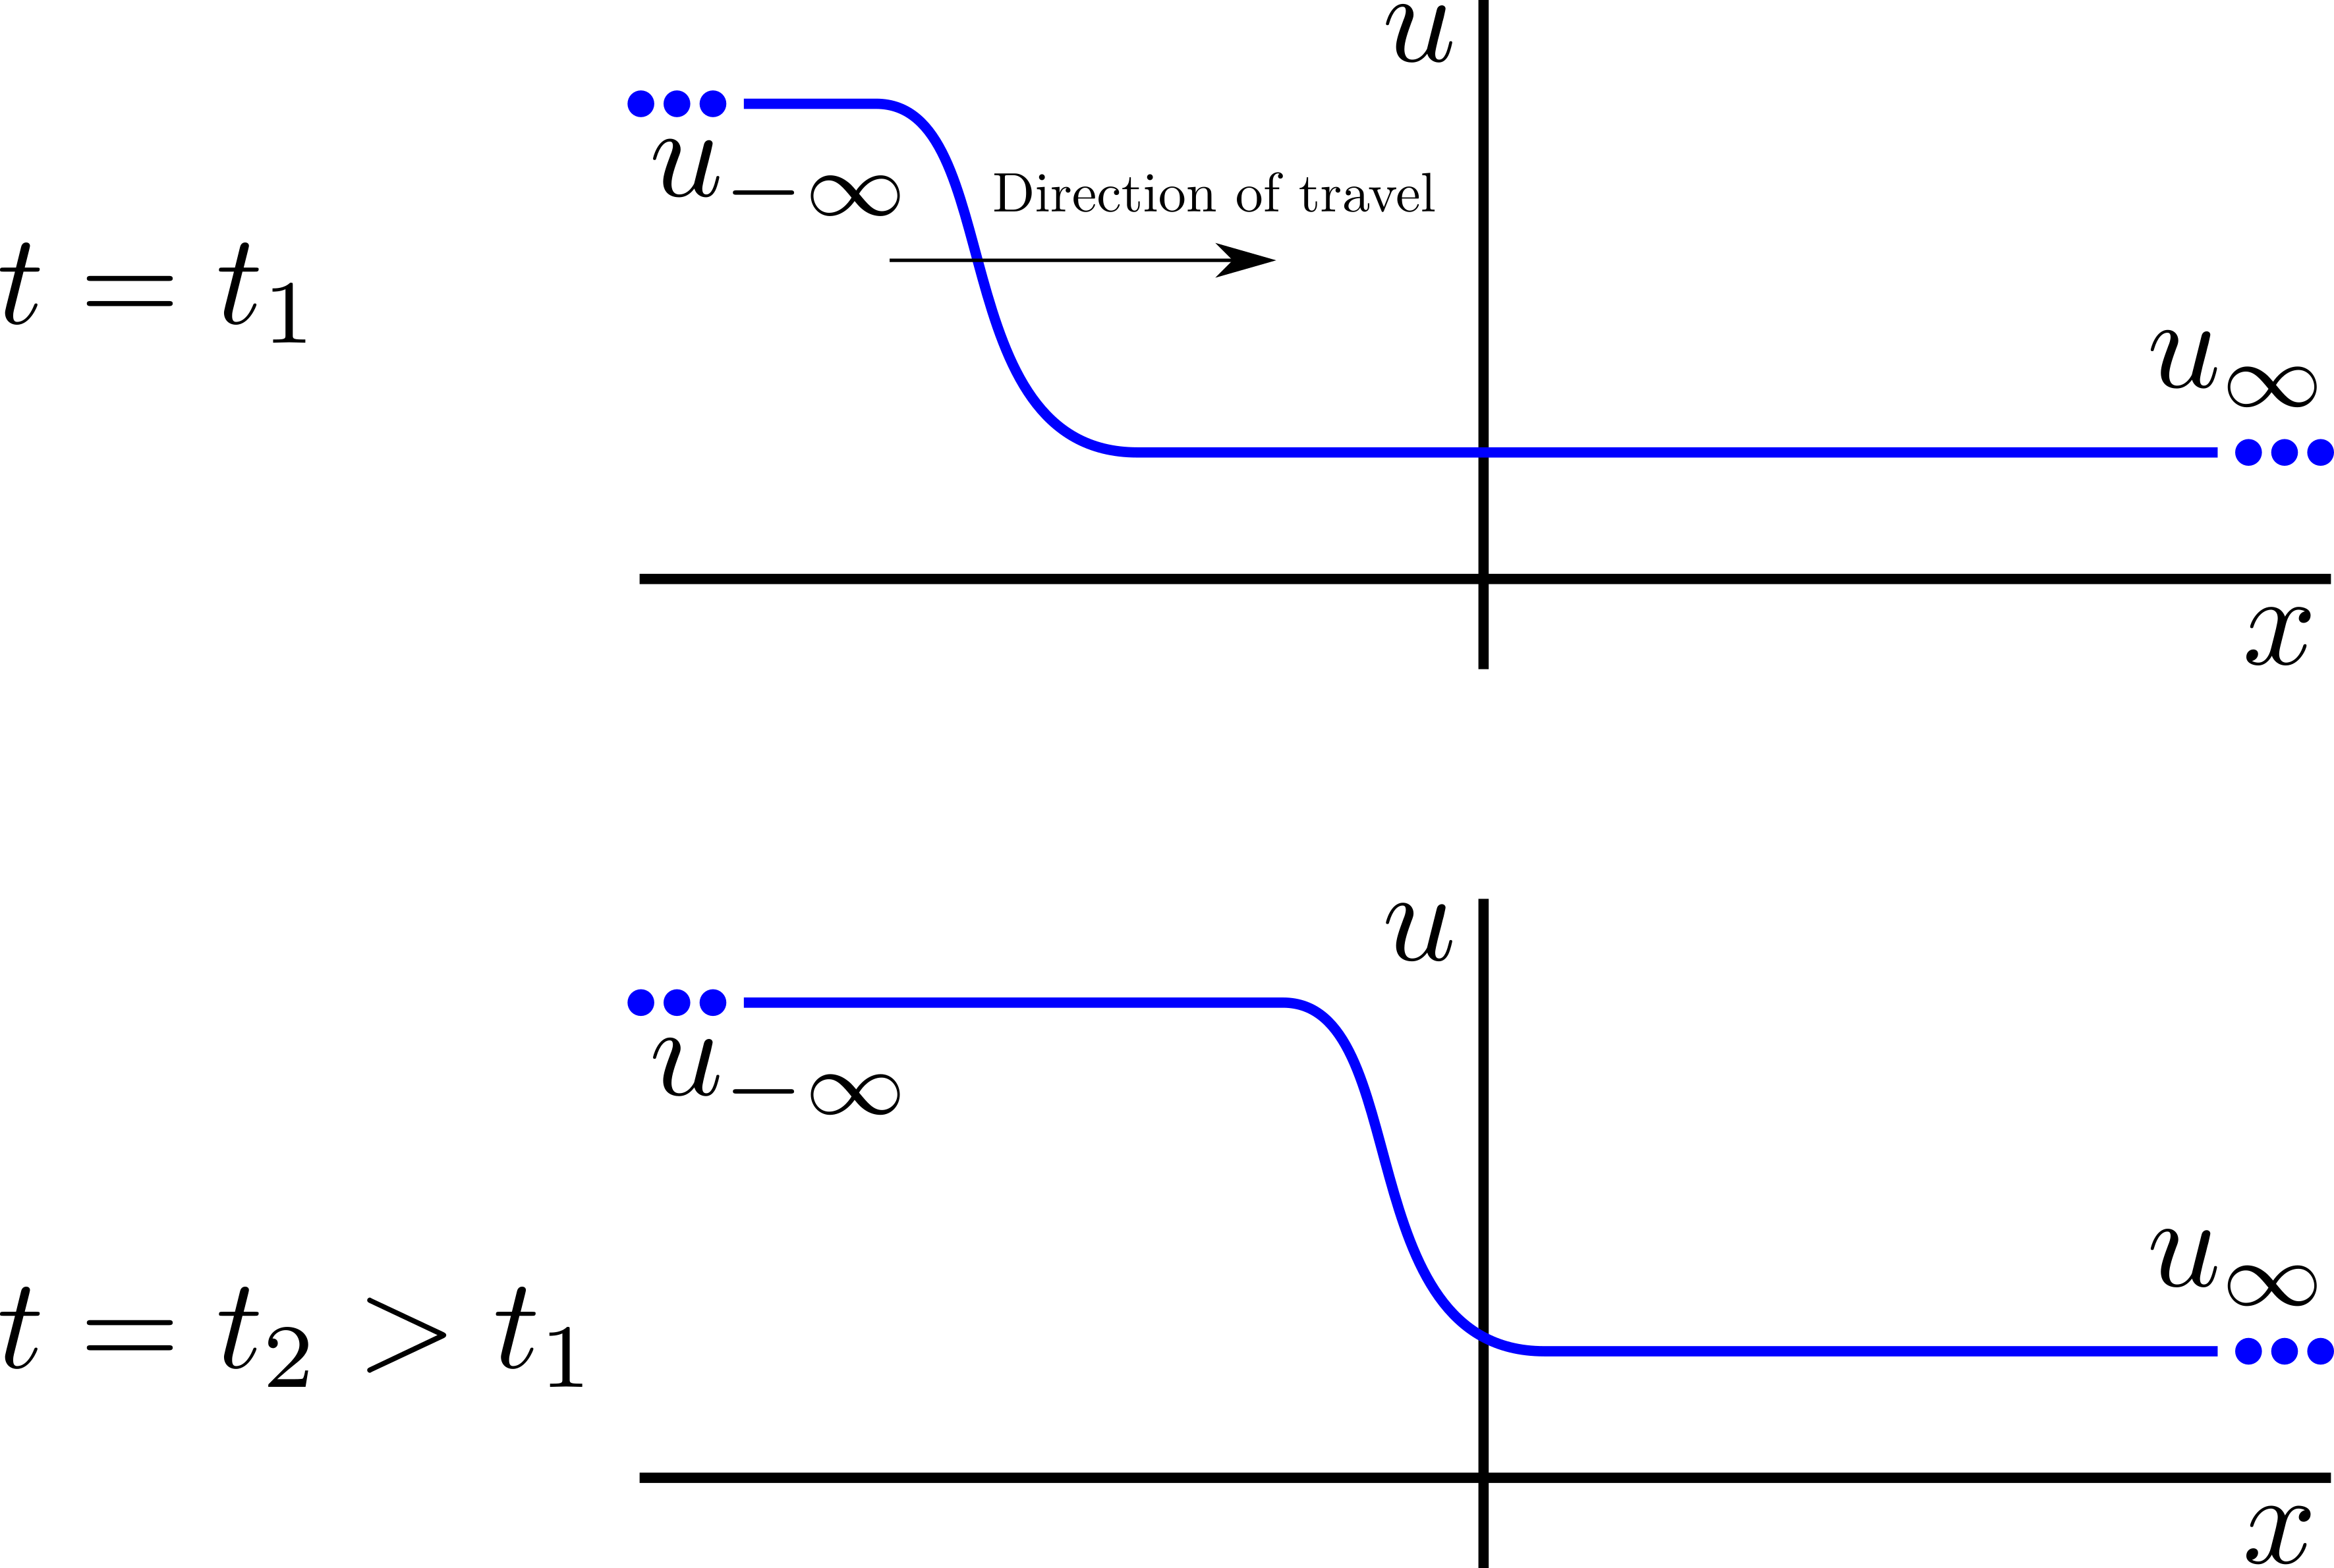
\includegraphics[width=0.7\textwidth]{../Pictures/Fisher_wave.png}
\caption{\label{Fisher_wave_fig} Schematic diagram of what a Fisher wave should look like, to aid our intuition.}
\end{figure}
\begin{figure}[!!!h!!!tb]
\centering
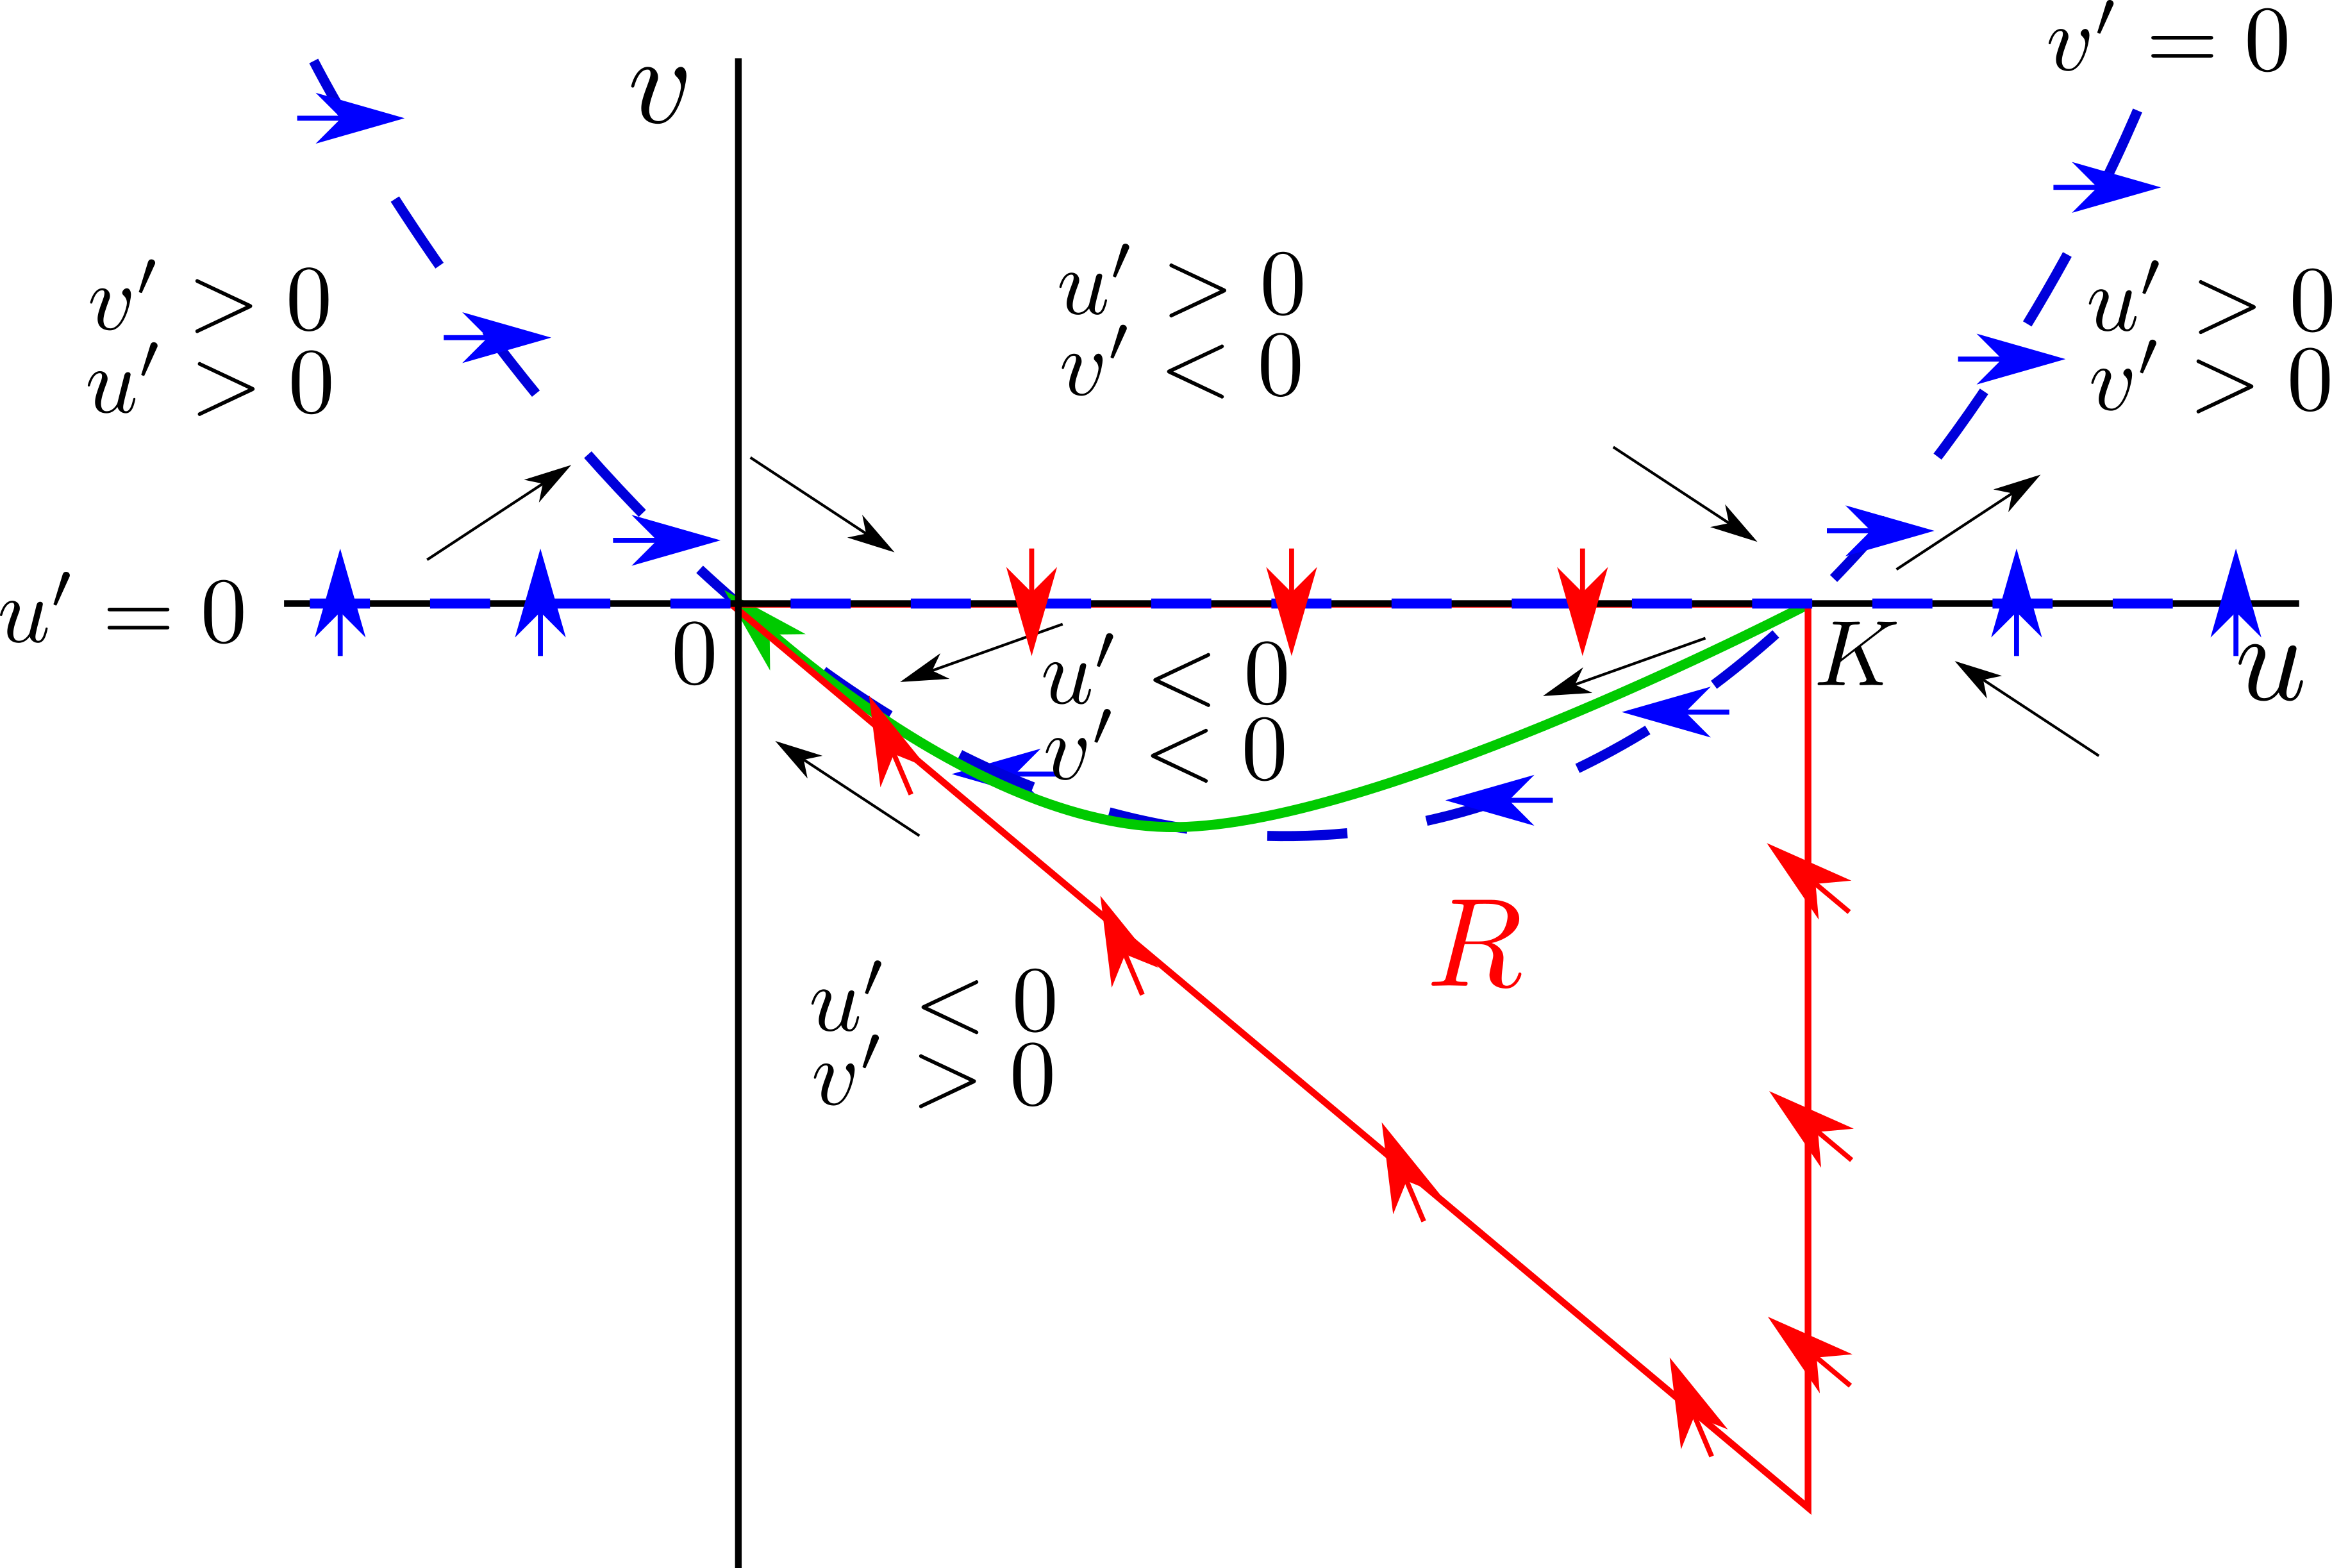
\includegraphics[width=0.7\textwidth]{../Pictures/Fisher_phase_plane.png}
\caption{\label{Fisher_phase_plane} Phase plane of the Fisher equation in moving coordinates, \eqns{Fisher_u}{Fisher_v}.}
\end{figure}
\begin{figure}[!!!h!!!tb]
\centering
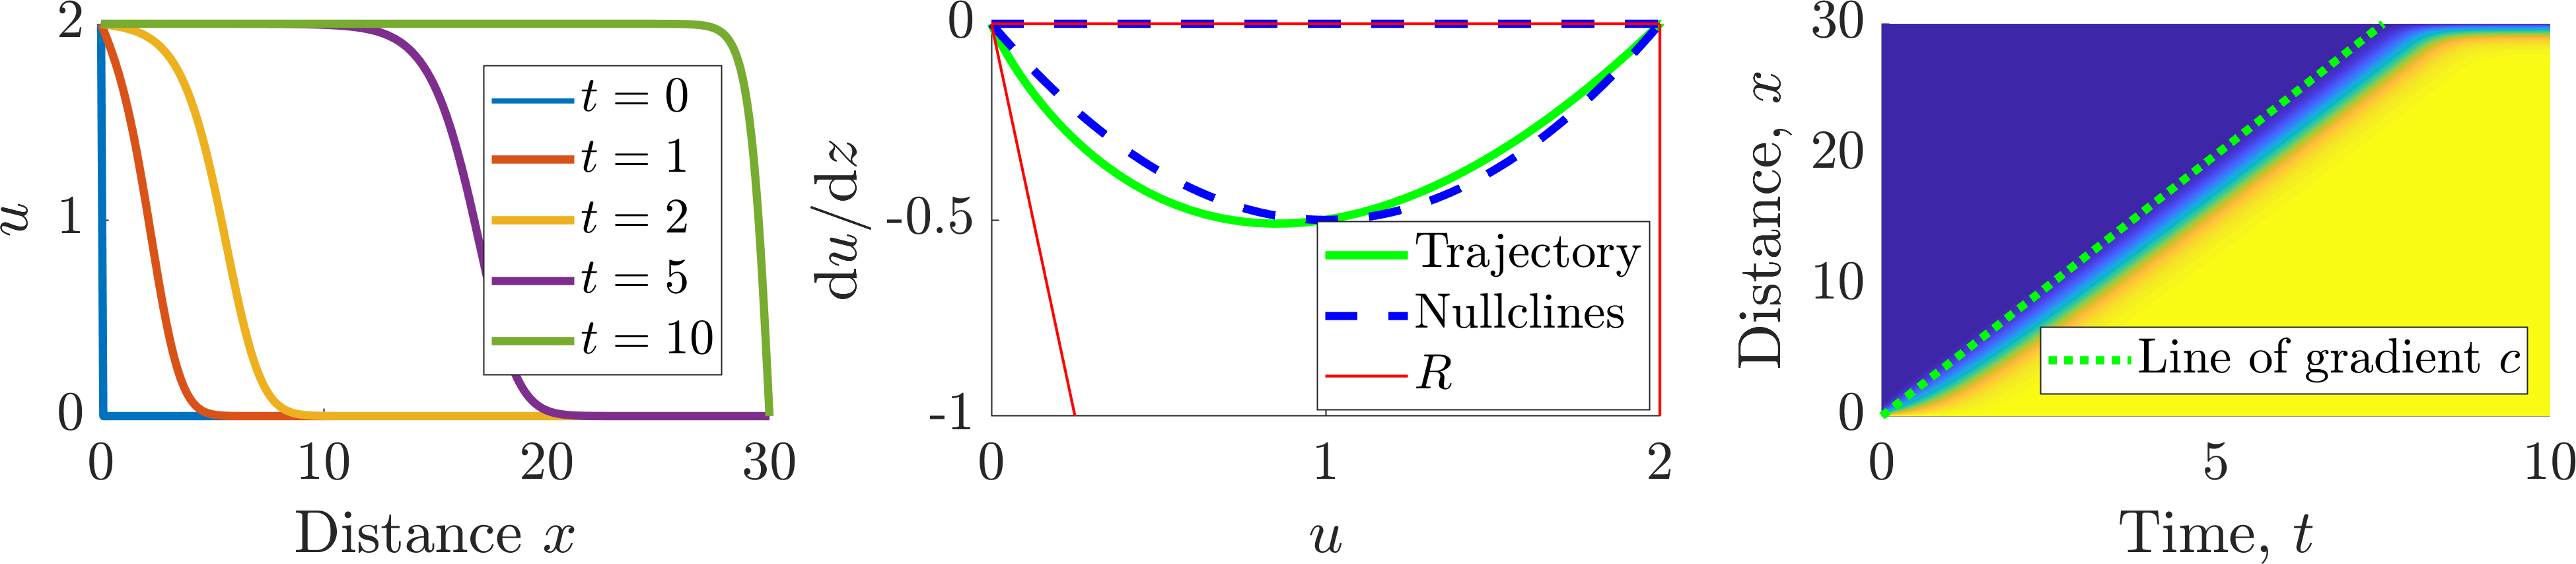
\includegraphics[width=\tp]{../Pictures/Fisher_sims.png}
\caption{\label{Fisher_sims} Simulation of Fisher's \eqn{Fisher} presented in a number of ways. Left: Different time points of the wave profile. Middle: Phase plane with added simulated trajectory. Right: Time-space plot of $u$. Parameters $r=4$, $D=1$ and $K=2$.}
\end{figure}
\section{Check list}
By the end of this chapter you should be able to:
\begin{todolist}
\item reproduce all definitions;
\item state and prove all theorems, where proofs are given;
\item derive the taxis and diffusion PDE forms from discretised domains;
\item derive appropriate boundary condition from discretised domains;
\item specify what different boundary conditions mean;
\item convert PDEs to travelling wave coordinates;
\item derive conditions underwhich travelling waves could form.
\end{todolist}
